\documentclass[specification,annotation]{itmo-student-thesis}

\usepackage{subcaption}

\newcommand{\revise}[1]{{\color{red!70!black} #1 }}

%% Опции пакета:
%% - specification - если есть, генерируется задание, иначе не генерируется
%% - annotation - если есть, генерируется аннотация, иначе не генерируется
%% - times - делает все шрифтом Times New Roman, требует пакета pscyr.

%% Указываем файл с библиографией.
\addbibresource{wjf-thesis.bib}

\begin{document}

\studygroup{M4236}
\title{Разработка эффективной структуры данных, поддерживающей инкрементальные изменения, для параллельной обработки деревьев}
\author{У Цзюньфэн}{У Цзюньфэн}
\supervisor{Станкевич Андрей Сергеевич}{Станкевич А.С.}{канд. техн. наук, без звания}{доцент кафедры компьютерных технологий Университета ИТМО}
\publishyear{2016}
\startdate{01}{сентября}{2014}
\finishdate{31}{мая}{2016}
\defencedate{20}{июня}{2016}

\addconsultant{Буздалов М.В.}{канд. техн. наук, без звания}

%% Задание
%%% Техническое задание и исходные данные к работе
\technicalspec{Требуется разработать структуру данных для параллельной обработки деревьев, поддерживающую инкрементальные изменения (добавление нового узла, подвешивание узла в качестве ребенка другого 
узла, отцепление узла от его родителя, изменение меток на вершинах и ребрах). В разработанной структуре данных требуется снять ограничение на максимальную 
степень вершины, имеющееся у существующих реализаций. Требуется поддержка эффективного выполнения запросов на определения корня дерева по представителю дерева,
определение групповой суммы меток в поддереве данной вершины и на пути между двумя данными вершинами. При этом требуется поддерживать произвольные типы меток на вершинах и ребрах, являющихся 
моноидами (произвольный моноид для ребер и коммутативный для вершин). Структуру данных требуется реализовать на языке C++ с использованием библиотеки PASL для реализации параллельных операций.}

%%% Содержание выпускной квалификационной работы (перечень подлежащих разработке вопросов)
\plannedcontents{\begin{enumerate}
    \item обзор источников с целью выявления наиболее перспективной структуры данных для поддержки операций с динамическими деревьями;
    \item реализация выбранной структуры данных в виде контейнера языка C++, 
          поддерживающего необходимые запросы и операции модификации;
    \item реализация эффективного параллельного применения пакетов модификаций;
    \item экспериментальные исследования эффективности разработанной реализации.
\end{enumerate}}

%%% Исходные материалы и пособия 
\plannedsources{\begin{refsection}
\nocite{sleator83,reif94,acar04}
\printannobibliography
\end{refsection}}
%%% Календарный план
\addstage{Изучение исходных материалов и пособий}{ноябрь 2014}
\addstage{Разработка программного интерфейса для реализации параллельных динамических 
деревьев}{февраль 2015}
\addstage{Реализация последовательного алгоритма}{июнь 
2015}
\addstage{Реализация ядра параллельного алгоритма}{ноябрь 2015}
\addstage{Реализация параллельных операций с помощью библиотеки PASL}{декабрь 2015}
\addstage{Реализация параллельных операций с помощью альтернативной библиотеки}{декабрь 2015}
\addstage{Экспериментальные исследования и доработка параллельных алгоритмов}{апрель 2015}
\addstage{Оформление магистерской диссертации}{май 2015}

%%% Цель исследования
\researchaim{Разработка структуры данных на основе Rake-and-Compress деревьев для параллельной обработки деревьев, поддерживающей инкрементальные изменения: добавление нового узла, подвешивание узла в 
качестве ребенка другого узла, отцепление узла от его родителя, изменение меток на вершинах и ребрах.}

%%% Задачи, решаемые в ВКР
\researchtargets{\begin{enumerate}
    \item снятие ограничения на число детей вершины, присущее параллельным реализациям Rake-and-Compress деревьев;
    \item уменьшение использования памяти с $\Theta(n \log n)$ до $\Theta(n)$, где $n$~--- общее число вершин в деревьях, при сохранении эффективности параллельных операций;
    \item обеспечение поддержки меток произвольных типов для вершин и ребер, при условии что метки на вершинах являются элементами коммутативного моноида, а метки на ребрах~---
          элементами произвольного моноида.
\end{enumerate}}

%%% Использование современных пакетов компьютерных программ и технологий
\advancedtechnologyusage{В реализации был использован язык C++ стандарта C++11. Для обеспечения целостности и надежного хранения кода использовалась система контроля версий Git.
Для реализации параллельных операций использовалась библиотека Parallel Algorithm Scheduling Library (PASL).}

%%% Краткая характеристика полученных результатов 
\researchsummary{Разработана эффективная реализация Rake-and-Compress деревьев. Ограничение на число детей вершины снято путем раздваивания каждой вершины и
организации декартова дерева для детей каждой вершины. Использование памяти уменьшено до $\Theta(n)$ при сохранении эффективности параллельных операций
путем хранения вершин в контейнерах переменной длины (векторах) отдельно для четных и нечетных раундов сжатия Rake-and-Compress деревьев, что позволило разделить
области памяти для чтения и для записи различными потоками.}

%%% Гранты, полученные при выполнении работы 
\researchfunding{гранты отсутствуют.}

%%% Наличие публикаций и выступлений на конференциях по теме выпускной работы
\researchpublications{
\begin{refsection}
По теме выпускной работы были сделаны выступления на двух всероссийских конференциях, по итогам которых
имеются следующие публикации:\nocite{wjf-kmu, wjf-spisok}
\printannobibliography
\end{refsection}
}

%% Эта команда генерирует титульный лист и аннотацию.
\maketitle{Магистр}

%% Оглавление
\tableofcontents

%% Макрос для введения. Совместим со старым стилевиком.
\startprefacepage

Структуры данных для поддержания динамических деревьев имеют прямое приложение к эффективному решению многих практическим задач,
таких как поиск максимального потока~\cite{goldberg88}. Такие структуры данных должны поддерживать лес деревьев на заданных вершинах,
операции обновления (добавление и удаление ребер, а в случае укорененных деревьев~--- подвешивание вершины к вершине и отцепление вершины).
Также, как правило, на вершинах, ребрах, или и тех, и других имеются пометки. Структуры данных также должны уметь отвечать на запросы
вида <<достижима ли вершина $A$ из вершины $B$ по ребрам деревьев>>, <<найти длину пути из вершины $A$ в вершину $B$>>,
<<найти сумму пометок на пути из вершины $A$ в вершину $B$>>, <<найти сумму пометок в поддереве вершины $A$>> и другие.
С практической точки зрения, полезно также уметь строить такие структуры данных параллельно,
а также параллельно применять совокупности, или пакеты, операций обновления.

Впервые задача поддержания динамических деревьев была поставлена в работе Слейтора и Тарьяна~\cite{sleator83}, в которой была предложена
структура данных, известная сейчас как ST-дерево или Link-Cut дерево. Эта структура данных поддерживает операции добавления и удаления ребер.
Также она поддерживает пометки на ребрах и запросы вида <<найти сумму пометок на пути из одной вершины в другую>>.

В то же время в ряде работ~\cite{miller85, miller89, miller91, reif94} Миллером и Рейфом был разработан подход параллельной обработки деревьев,
известный как <<параллельное сжатие деревьев>> (англ.~Parallel Tree Contraction). Суть этого подхода заключается в построении структуры данных,
описывающей данное дерево и позволяющей выполнять запросы различного вида на этом дереве, таким образом, чтобы основная часть работы выполнялась
параллельно. Тем самым, при наличии многопроцессорных вычислительных систем, сокращается время между получением входных данных и моментом, начиная
с которого возможно эффективное выполнение запросов к дереву.

Различные варианты параллельного сжатия деревьев применяются для реализации динамических деревьев для ускорения применения изменений при наличии
многопроцессорных вычислительных систем. Так, известны структуры данных Topology Trees~\cite{frederickson97}, Top Trees~\cite{alstrup05} и RC-Trees~\cite{acar03},
поддерживающие параллельное построение, при этом 
некоторые из них также поддерживают применение различных операций модификации, в том числе параллельно. 
В работе~\cite{acar04} исследовалась возможность добавления поддержки инкрементальных изменений дерева путем привнесения идей
из работы~\cite{miller85}. В то же время, эти структуры накладывают различные ограничения на вид поддерживаемого дерева или на поддерживаемые операции модификации.

\paragraph{Мотивация.}

Задача поддержки динамических деревьев все еще не может считаться решенной удовлетворительно. Так, многие из существующих структур данных не поддерживают параллельное
обновление, работу с метками на ребрах или на вершинах, агрегационные запросы на путях или поддеревьях, или работу с деревьями, имеющими вершины произвольной степени.
Остается открытым также вопрос эффективной реализации таких структур данных~--- в частности, по времени выполнения запросов, времени применения операций обновления,
используемой памяти, использованию кешей различных уровней, эффективности использования ядер многопроцессорных систем.

Кроме того, для структур данных, поддерживающих параллельное построение или обновление, отсутствуют их реализации, удобные для использования в приложениях.
Существующие программные реализации имеют исключительно исследовательский характер и трудны для переиспользования, в то время как для пользователей
была бы удобна реализация, устроенная по образцу контейнеров или коллекций из стандартных библиотек языков программирования (таких как
\texttt{std::vector} в \emph{C++} или \texttt{java.util.ArrayList} в \emph{Java}).

Контейнерную реализацию дополнительно усложняет тот факт, что использование отложенного обновления (в том числе параллельного) требует от структуры данных
поддержки в том или ином виде минимум двух версий данных~--- последней стабильной версии и текущей версии, содержащей еще не примененные изменения.
В дополнение к этому, вновь применяемые изменения крайне желательно проверять на корректность, причем в некоторых случаях такая проверка может занимать большую часть
времени работы со структурой данных, поэтому также требуется предусмотреть режим, в котором корректность не проверяется.

Наличие указанных проблем мотивируют создание эффективной реализации структуры данных, поддерживающей параллельное применение пакетов изменений,
реализованной в виде переиспользуемого обобщенного контейнера данных, поддерживающего опциональную проверку корректности применяемых изменений.

\paragraph{Цели исследования.}

В настоящей диссертации, оцениваются преимущества структуры данных RC-Trees и анализируются требованию к разработке новой структуры данных на 
основе RC-Trees для решения динамических задач.

Целью данной диссертации является разработка и реализация эффективного параллельного алгоритма для сжатия дерева, поддерживающего инкрементные изменения 
данных. Для этого необходимо улучшить базовую структуру данных RC-Tree для поддержки коммутативных и некоммутативных данных, а также направленной и 
ненаправленной функций. Также требуется разработать параллельный алгоритм и оценить его эффективность. Для решения динамических задач в параллельных вычислениях 
в данной работе были использованы библиотеки OpenMP и PASL (Parallel Algorithm Scheduling Library).

Основной проблемой исследования является то, что неясно какую структуру данных следует использовать для достижения поставленных целей и какие ограничения 
на нее налагаются?
Второй проблемой исследования является то, что какой алгоритм, основанный на разработанной структуре данных позволяет поддерживать динамические деревья?

\paragraph{Ожидаемые результаты.}

Задачи для которых применяются алгоритмы параллельного сжатия дерева, описанного в диссертации, могут быть использованы для оценки эффективности 
используемой структуры данных. Одной из задач, которая может быть решена с помощью алгоритма параллельного сжатия дерева является Change 
propagation~\cite{acar05}.
Change propagation автоматически адаптирует выходные данные алгоритма к изменению входных. Другой задачей, которая решается алгоритмом сжатия дерева 
является вычисление выражений. Параллельное выполнение сжатия дерева могло бы сделать вычисления более эффективными.

Ожидаемыми результатами этой диссертации являются разработка новой структуры данных на основе RC-Tree, поддерживающей требуемый тип данных. Эффективность новой 
структуры данных должна быть приемлемой для последовательных вычислений. Должна существовать возможность установки максимального времени вычисления для ответа 
на запрос. Также должны быть возможности последовательного и параллельного, с использованием OpenMP и PASL, выполнения. Также дожна быть возможность оценки 
эффективности с использованием различных вычислительных типов. При параллельной работе алгоритм должен отвечать на запросы быстрее, чем при последовательной 
обработке, иначе разработка параллельного алгоритма не имеет смысла.

Таким образом, ожидаемым результатом является разработка и реализация улучшенной версии базовой структуры данных, эффективность которой удовлетворяет 
требованиям диссертации.

%% Начало содержательной части.
\chapter{Обзор источников}

В данной главе приведен обзор литературных источников, используемых в настоящей работе. 
В разделе~\ref{survey-tree} описывается задача поддержания динамических деревьев и известные структуры данных для решения этой задачи.
В разделе~\ref{survey-contraction} описываются алгоритмы параллельного сжатия деревьев.
В разделе~\ref{survey-misc} описываются вспомогательные алгоритмы и структуры данных, которые будут использованы при решении задач, поставленных в настоящей диссертации.

\section{Методы решения задачи поддержания динамических деревьев}\label{survey-tree}

Структуры данных для поддержания динамических деревьев имеют прямое приложение к эффективному решению многих практическим задач,
таких как поиск максимального потока~\cite{goldberg88}. Такие структуры данных должны поддерживать лес деревьев,
операции обновления (добавление и удаление ребер, а в случае укорененных деревьев~--- подвешивание вершины к вершине и отцепление вершины).
Также, как правило, на вершинах, ребрах, или и тех, и других имеются пометки. Структуры данных также должны уметь отвечать на запросы
вида <<достижима ли вершина $A$ из вершины $B$ по ребрам деревьев>>, <<найти длину пути из вершины $A$ в вершину $B$>>,
<<найти сумму пометок на пути из вершины $A$ в вершину $B$>>, <<найти сумму пометок в поддереве вершины $A$>> и другие.
С практической точки зрения, полезно также уметь строить такие структуры данных параллельно, а также параллельно применять совокупности, или пакеты, операций обновления.

\subsection{Link-Cut Trees}

ST-Tree является лучшей известной структурой данных для решения динамических задач, предложенной Sleator D D, Tarjan R E. (1983). Важными операциями этой 
структуры данных являются link и cut. Поэтому такая структура данных также известна как link-cut tree.

ST-Trees совершают операции на корневом дереве. В ST-Trees вводятся три операции: операция link (v, w), которая соединяет корневую вершину v и вершину w из 
другого дерева, добавляя ребро (v, w) и делая w родителем v; операция cut(v) удаляет ребро между некорневой вершиной v и его родителем, затем разделяет дерево 
на два дерева; операция evert (v) делает вершину v корнем, поворачивая дерево относительно вершины v. Операции с ST-Trees изображены на 
рисунке~\ref{fig:link-cut-tree}.

\begin{figure}[!ht]
\centering
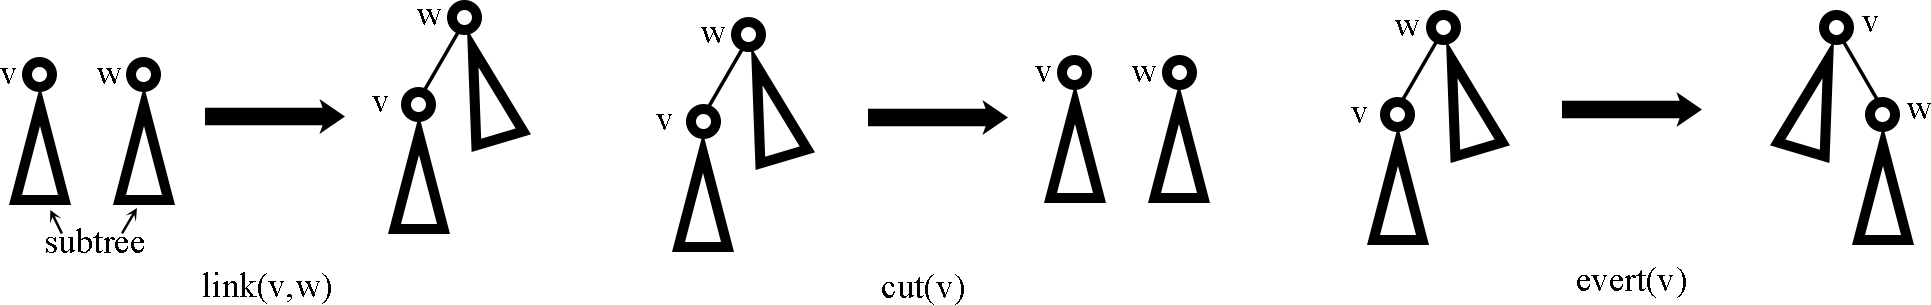
\includegraphics[width=\textwidth]{pic/link-cut-tree.png}
\caption{Операции Link-Cut деревьев: \texttt{Link}($v$, $w$), \texttt{Cut}($v$), \texttt{Evert}($v$)}\label{fig:link-cut-tree}
\end{figure}

ST-Trees поддерживают операции пути, требующие $O(\log n)$ времени на одну операцию на 
сбалансированном дереве в худшем случае, и амортизированно $O(\log n)$ времени 
на одну операцию на несбалансированном дереве. ST-Trees может также поддерживать другие запросы, но информация должна агрегироваться только над путями. 
ST-Trees является первой структурой данных в которой динамические запросы выполняются за логарифмическое время. Поэтому структуры данных для решения 
динамических задач основываются ST-Trees. 

\subsection{Topology Trees}

Первой структурой данных, основанной на сжатии, является Topology Tree, которую ввел Frederickson, G. N. (1997). Topology Tree является деревом поддержки.
Рассмотрим дерево сжатия S на основе дерева T. Каждый узел в S является поддеревом в T, и кластер сжатия дерева T является поддеревом, соответствующим узлу в 
S. Пример топологического дерева представлен на рисунке~\ref{fig:topology-tree}. Вверху изображено дерево T, под ним представлено дерево Т', являющегося 
кластером сжатия S. Ребро в Т соответствует инцидентному ребру Т'. Степенью кластера Т' является число инцидентных ребер. Вершина кластера Т' из S является 
граничной вершиной, если она имеет инцидентное ребро. Число граничных вершин кластера Т' является размером его граница (Acar U.et al. 2003).

\begin{figure}[!ht]
\centering
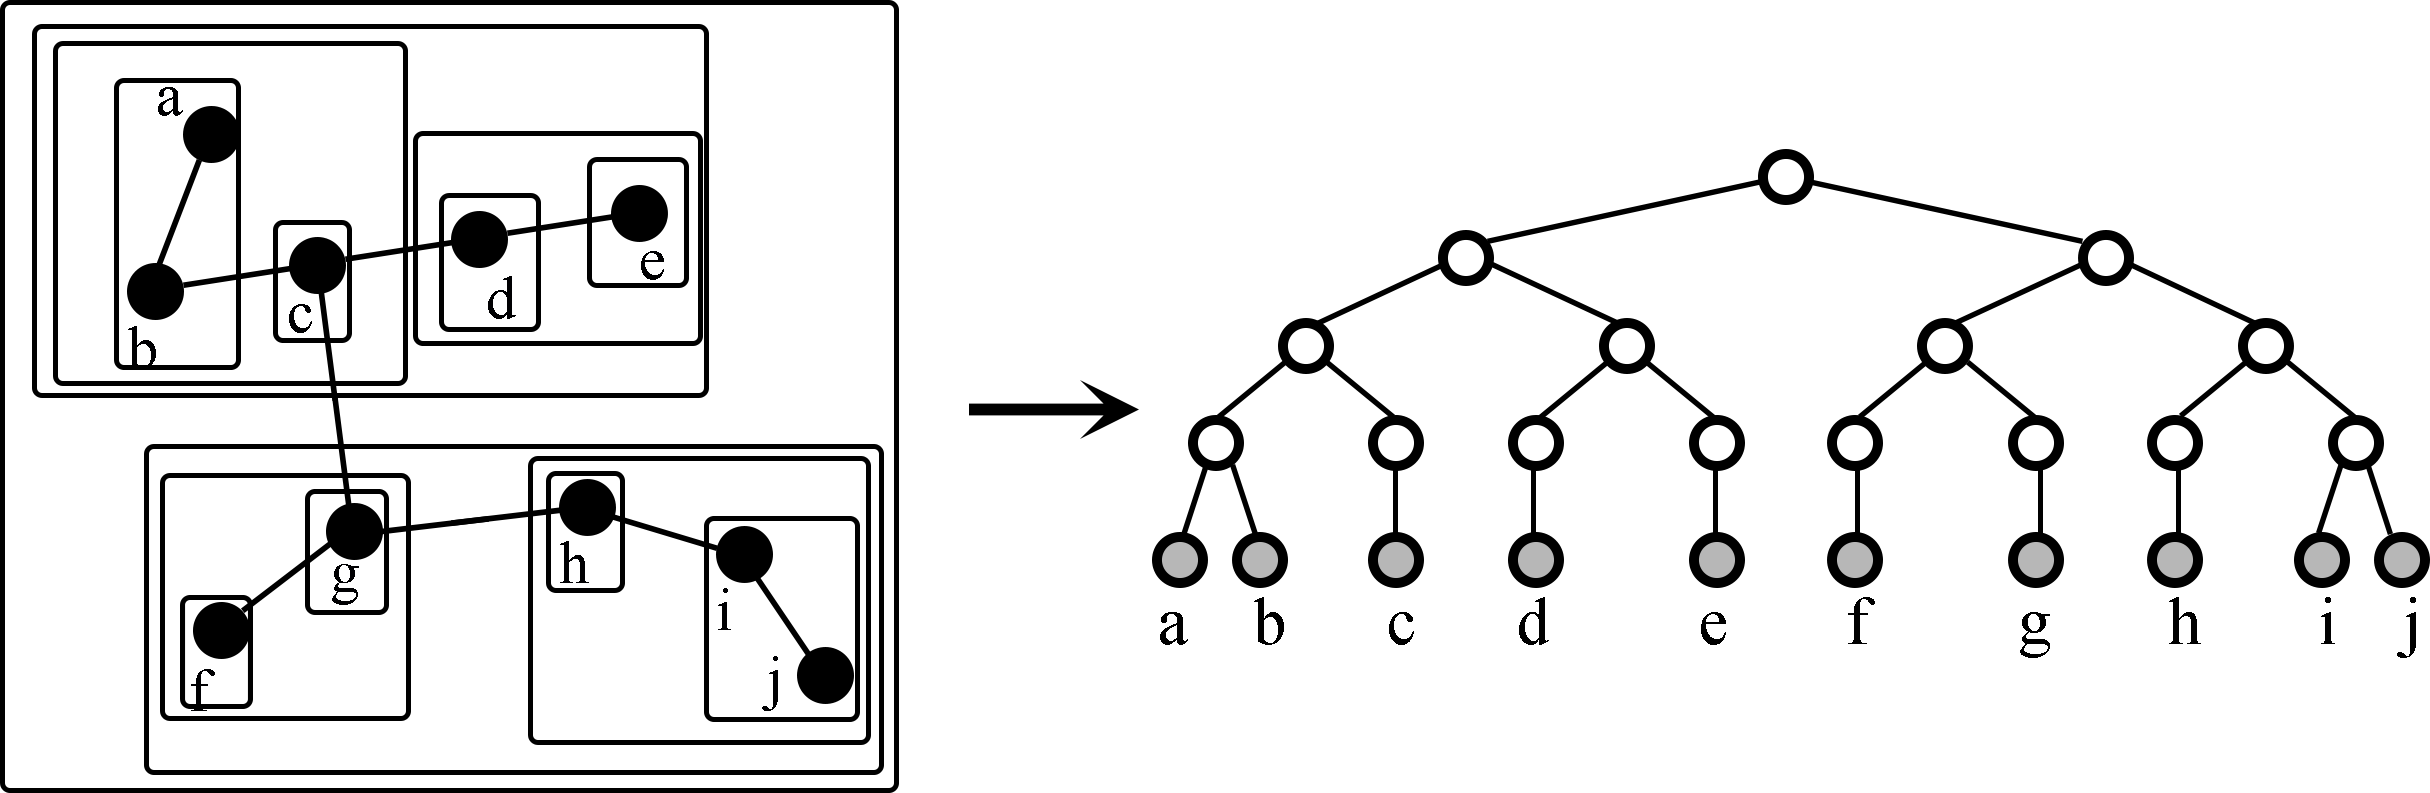
\includegraphics[width=\textwidth]{pic/topology-tree.png}
\caption{Пример Topology Tree}\label{fig:topology-tree}
\end{figure}

Frederickson, G. N. (1997) предложил интерпретировать кластеры как вершины вместо ребер в качестве дерева поддержки. В Topology Trees, кластер имеет не более 
трех степений. Направленная структура данных Topology Trees разработана для поддержания динамических бинарных деревьев. Время работы операции в таких 
деревьях занимает $O(\log n)$, где $n$ является количеством вершин в деревьях. Topology Trees 
являются реализацией link-cut trees, так что основными операциями в 
Topology Trees также являются link и cut. Хотя Topology Trees упрощают сжатие динамического дерева с точки зрения алгоритма, требование что степень всех вершин 
в лесу ограничена константой, ограничивает разработку. Для более эффективной работы алгоритма, структура данных должна поддерживать изменяемую 
степень вершин в дереве поддержки.

\subsection{Top Trees}

Структура данных Top Trees представляет собой структуру данных разработанную на основе двоичного дерева для некорневых динамических деревьев (Alstrup S. et 
al. 1997). В некорневом дереве, ребра, смежные с каждой вершиной произвольно расположены в фиксированном круговом порядке. Кластером в Top Trees является 
поддерево пути первоначального базового дерева. В Top Trees кластеры имеют размер не более двух. 
Операция сжатия занимает $O(\log n)$ времени, и преимущество 
состоит в том, что время не зависит от степени дерева. Ограничением Top Trees является то, что она поддерживает только бинарные деревья.

Сжатие дерева состоит в том, чтобы соединить все кластеры в дереве поддержки в единый кластер. Top Trees поддерживает операцию сжатия для бинарного дерева. 
Два кластера (u, v) и (v, w) могут быть объединены, если v является общей вершиной этих двух кластеров и имеет степень равную двум. Alstrup S. et al. (1997) 
использует понятие компресса, объединенный кластер (u, w) из двух кластеров называется компрессом кластера. Затем, если (w, x) является преемником (v, x) и v 
имеет степень один, эти кластеры могут быть объединены в объединенный кластер. После комбинации, объединенный кластер имеет граничные вершины w и x. 
Каждый объединенный или компресс кластер может рассматриваться как родитель, который агрегирует информацию, содержащуюся в ее детях. Корень верхнего дерева 
представляет собой кластер, который полностью лежит в основе дерева. При динамических изменениях лежащего в основе дерева, например, при применении 
операций link или cut, структура данных обновляет сжатие.

Структура данных Top Trees позволяет отвечать на динамические запросы. При выполнении путевого запроса, запрашивается путь между вершиной v и w, 
затем выполняется операция expose (v, w), которая возвращает корневой кластер с вершинами v и w в качестве конечных вершин, а в случае если v и w находятся в 
разных деревьях, операция будет возвращать нуль. Однако, даже если v и w находятся одном дереве, сжатие верхнего дерева может потребоваться изменить, потому 
что корневым кластером станет путь от v до w. Top Trees поддерживает агрегацию по путям или по деревьям напрямую. Они не требуют определенную степень вершины, 
в отличие от Topology Trees что является преимуществом.

\subsection{RC-Trees}

Структура данных Rake-and-Compress Tree~\cite{reif94}~--- одна из наиболее подходящих структур данных для решения задач настоящей диссертации,
теоретически поддерживающая параллельное построение и параллельное обновление (включая не только добавление и удаление листьев дерева, но и произвольные
подвешивания и отцепления вершин), а также запросы как на путях, так и на поддеревьях.

Идея Rake-and-Compress деревьев, в изложении для укорененных деревьев, заключается в следующем. Для дерева последовательно строится несколько <<уменьшенных>> копий дерева, причем $i$-тая копия получается
из $(i-1)$-ой применением ко всем допустимым вершинам одной из следующих операций:
\begin{itemize}
    \item Rake. Вершина, имеющая родителя и не имеющая детей, удаляются вместе с ребром, ведущим к родителю (рисунок~\ref{fig:rake}).
    \item Compress. Вершина, имеющая родителя и ровно одного ребенка, удаляется вместе со смежными ребрами, а вместо этого ребро проводится от ребенка удаляемой вершины к родителю этой вершины
          (рисунок~\ref{fig:compress}). При этом родитель не должен подвергаться операции Compress, а ребенок не должен подвергаться ни операции Compress, ни операции Rake.
\end{itemize}

\begin{figure}[!ht]
\centering
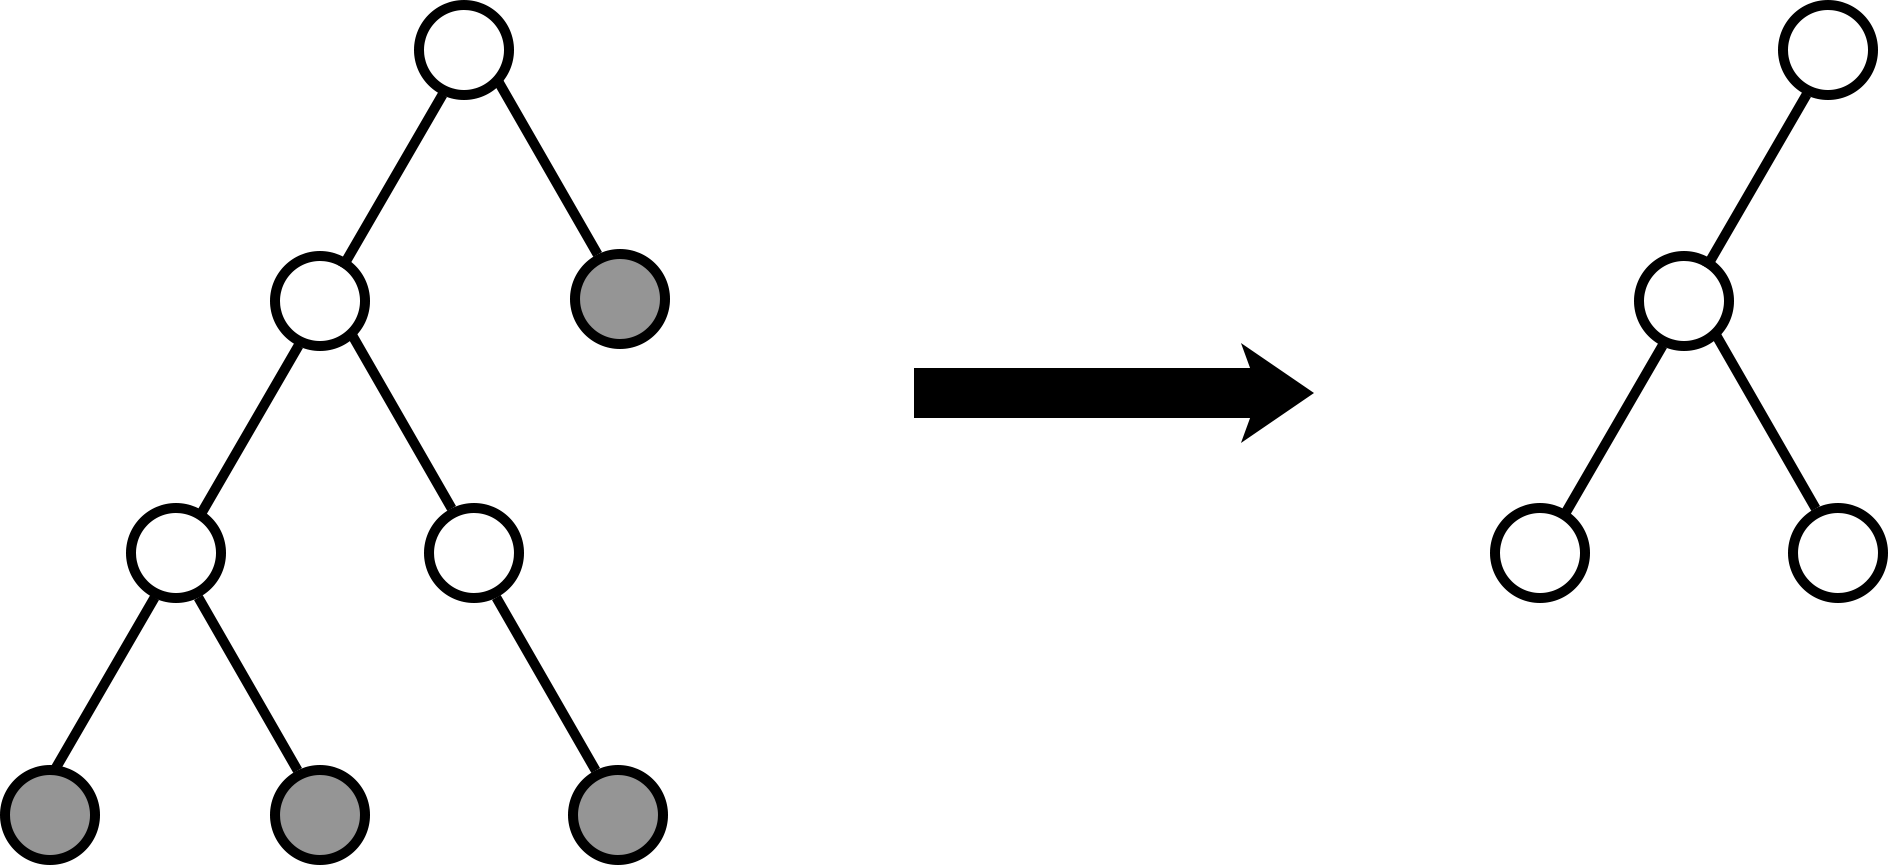
\includegraphics[width=0.5\textwidth]{pic/rake.png}
\caption{Операция Rake}\label{fig:rake}
\end{figure}
\begin{figure}[!ht]
\centering
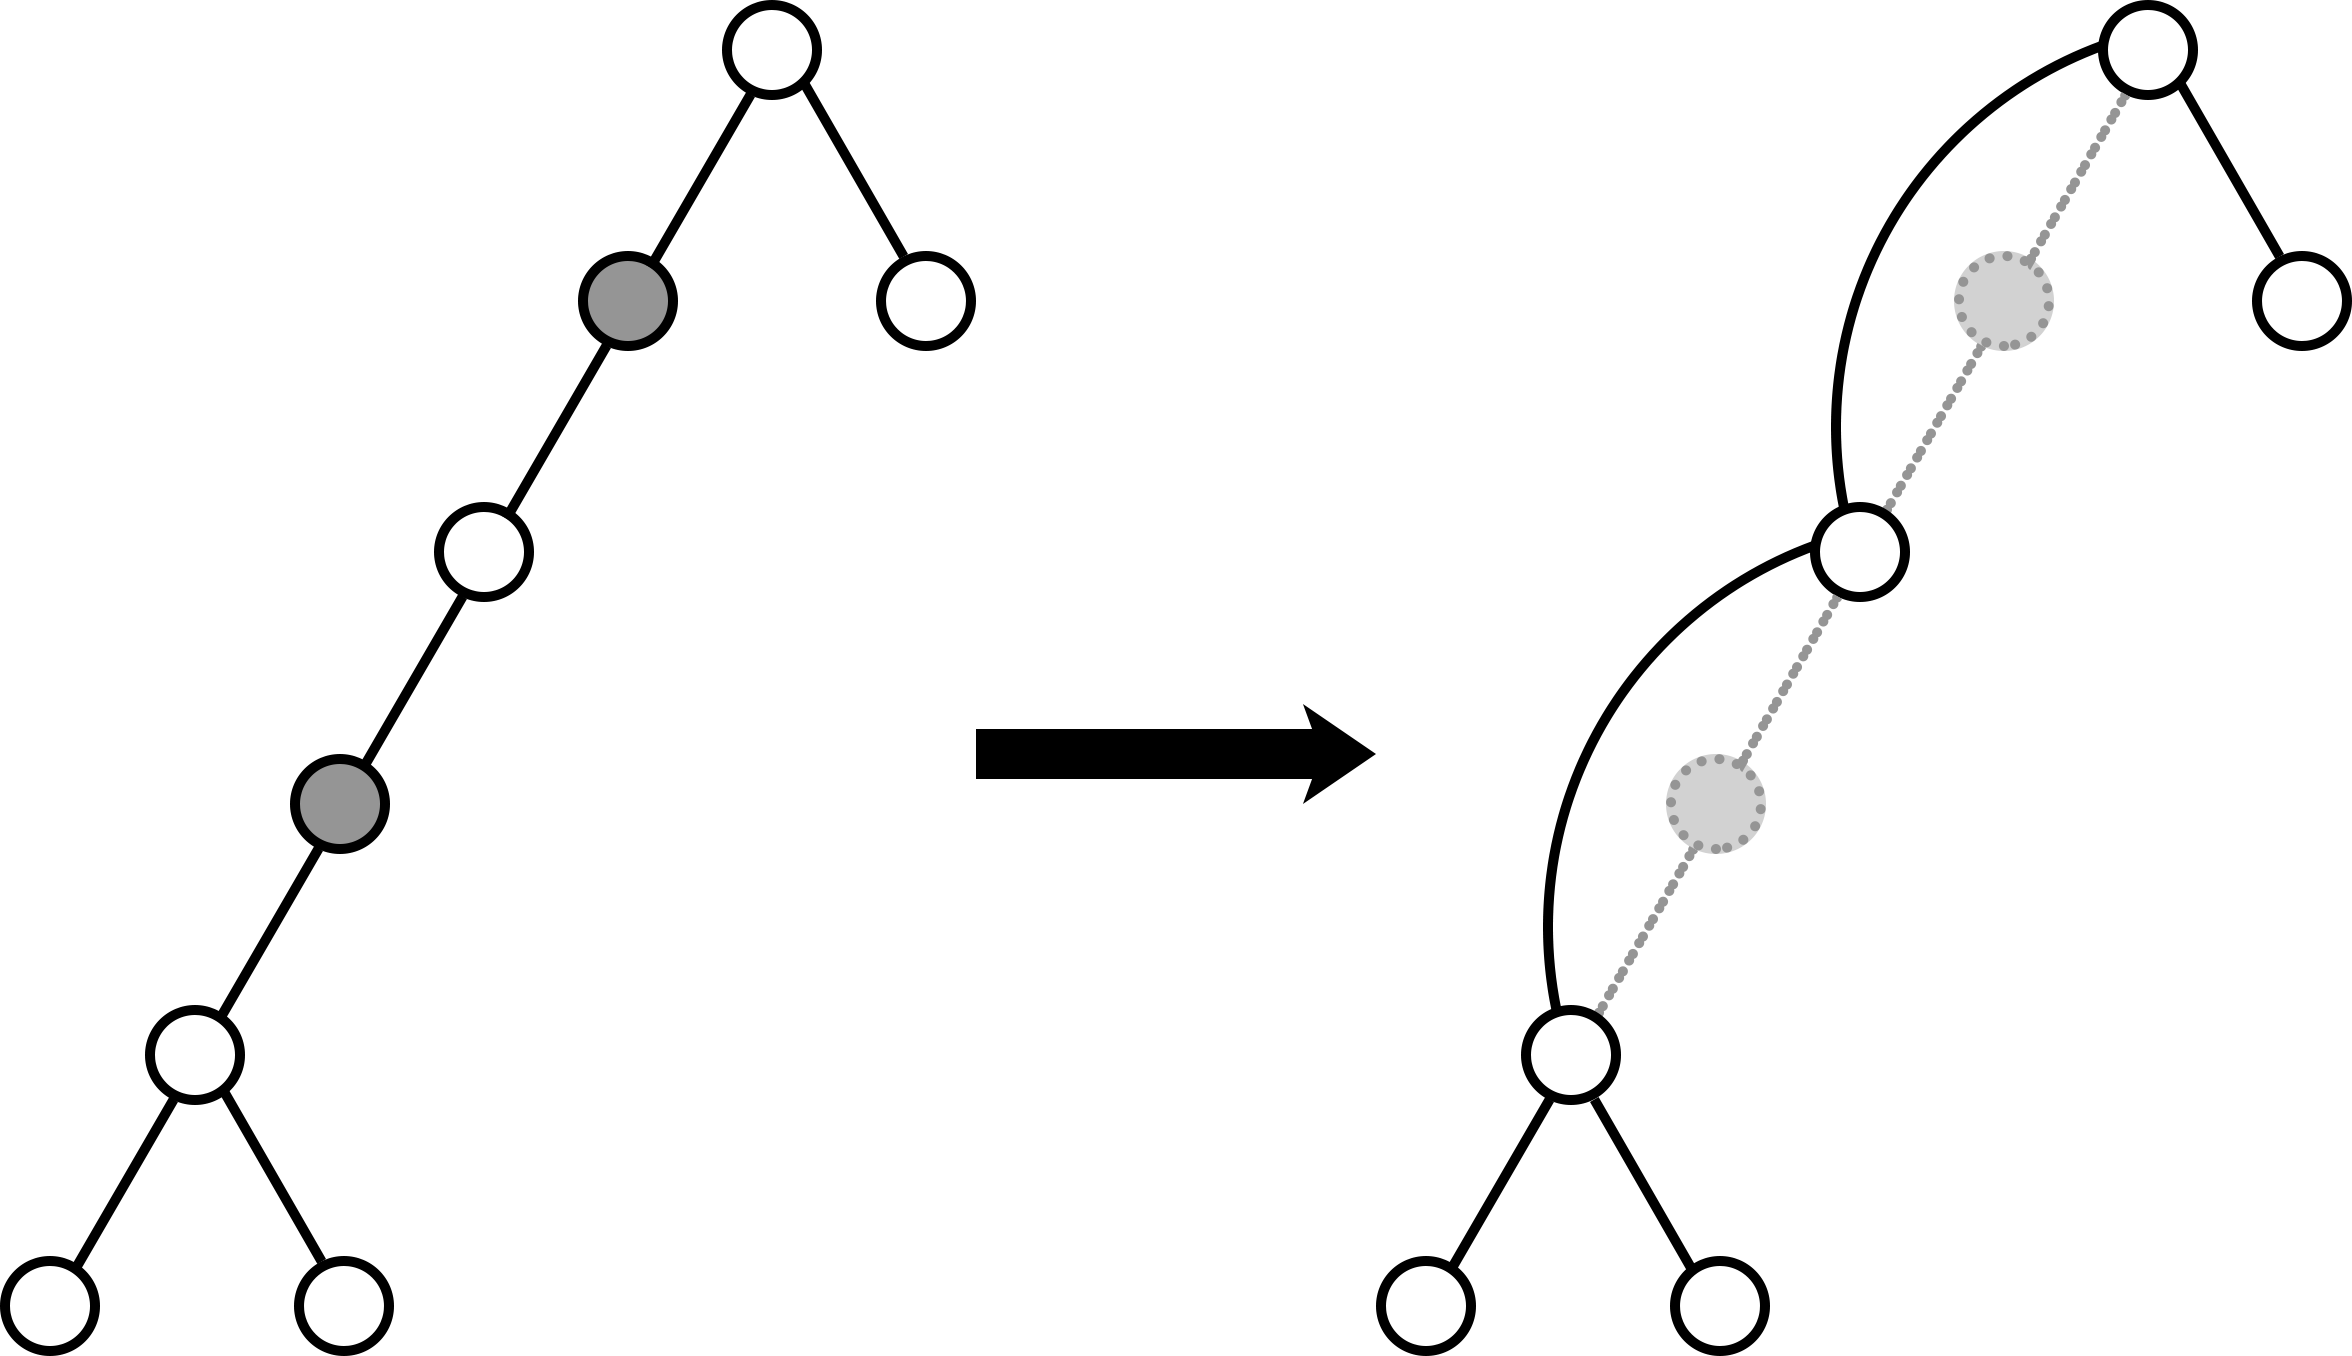
\includegraphics[width=0.5\textwidth]{pic/compress.png}
\caption{Операция Compress}\label{fig:compress}
\end{figure}

С каждым раундом число вершин в дереве, если оно больше единицы, уменьшается как минимум в $8/7$ раз в каждой компоненте связности. В конце работы для каждой компоненты связности
остается ровно одна вершина, для чего требуется произвести $O(\log n)$ раундов (рисунок~\ref{fig:rctree-overall}). RC-дерево можно представить как дерево с двумя типами вершин~--- первый тип соответствует 
вершинам оригинального дерева, второй тип~--- его ребрам (рисунок~\ref{fig:rctree-two-types}).

\begin{figure}[!ht]
\centering
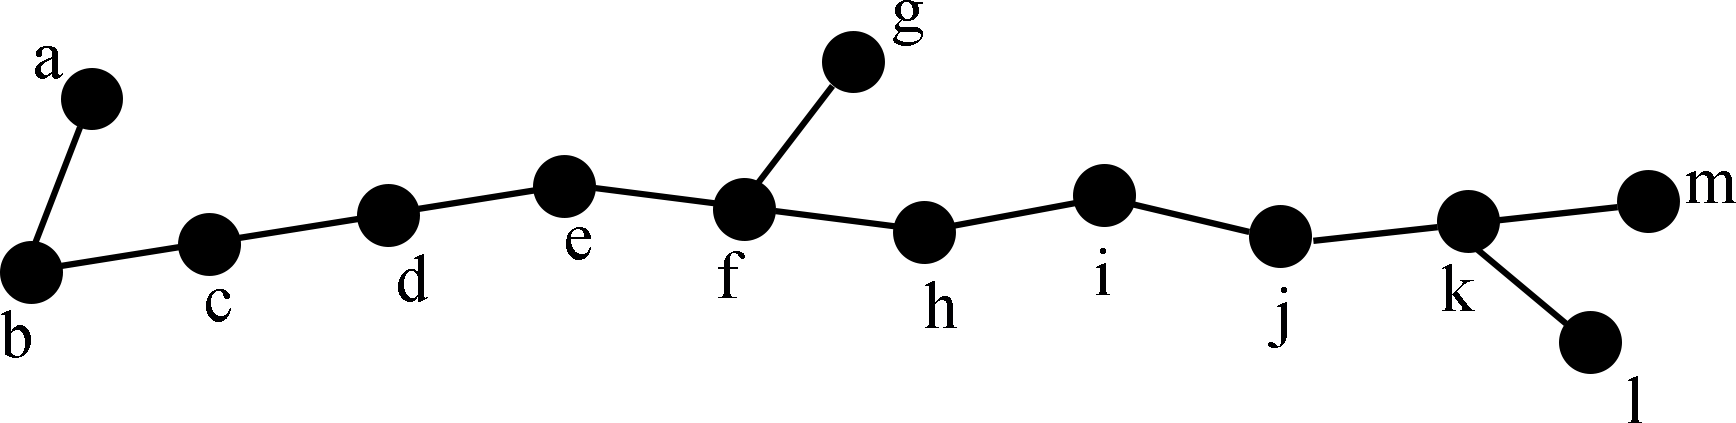
\includegraphics[width=0.5\textwidth]{pic/rc_tree_1_primitive_tree.png}\\

\includegraphics[width=0.75\textwidth]{pic/rc_tree_2_completed_clustering.png}
\caption{Исходное дерево и группировка вершин, полученная последовательным применением операций Rake и Compress}\label{fig:rctree-overall}
\end{figure}

\begin{figure}[!ht]
\centering
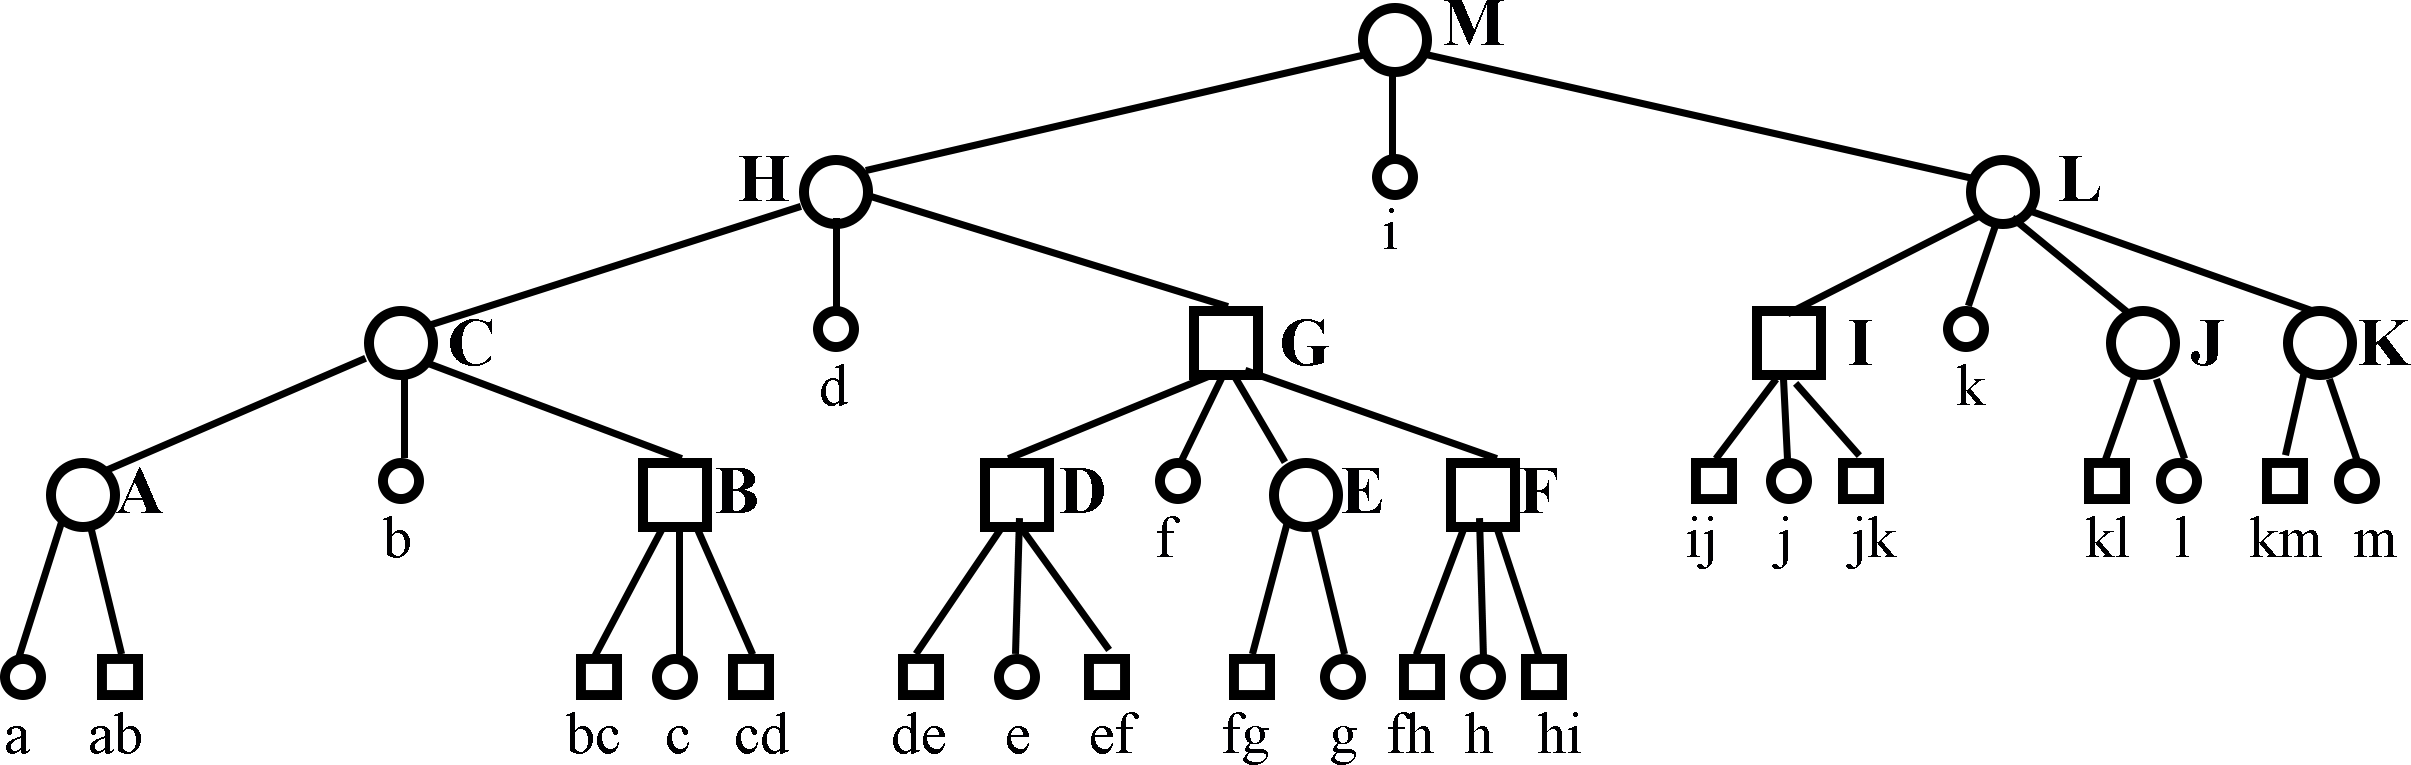
\includegraphics[width=\textwidth]{pic/rc_tree_4_two_types.png}
\caption{Представление RC-дерева как дерева с двумя типами вершин, соответствующим вершинам (круглые вершины) и ребрам (квадратные вершины) оригинального дерева}\label{fig:rctree-two-types}
\end{figure}

Такое многоуровневое представление дерева позволяет отвечать на запросы на путях и поддеревьях за время, пропорциональное числу раундов (а следовательно, $O(\log n)$),
даже если дерево изначально было несбалансировано (например, существенно вытянутое). В то же время решение о выполнении операции Rake или Compress можно сделать на основе локальной информации (о самой
вершине и ее ближайших соседях), что позволяет эффективно распараллеливать операции в рамках каждого раунда.
Эффективное применение операций обновления также возможно с использованием этой структуры данных~\cite{acar04}.

\section{Алгоритмы параллельного сжатия деревьев}\label{survey-contraction}

Динамические деревья решают предназначенные для них задачи последовательно. Тем не менее, сжатие дерева позволяет этим структурам данных 
работать более эффективно. Сжатием дерева является операция для уменьшения дерева путем удаления некоторых из узлов (Atallah, M. J. (Ed.). 1998). Чтобы 
операция сжатия дерева поддерживала изменяемые процессоры~\cite{miller85, miller89}, было введено параллельное сжатие дерева~\cite{miller91, reif94}. 
Фреймворк для параллельного сжатия дерева поддерживает эффективные параллельные алгоритмы на деревьях~\cite{morihata08}. Эффективный алгоритм параллельного 
сжатия дерева позволяет собирать значения в дереве эффективно и без конфликтов, что в результате, приводит к нескольким эффективным параллельным 
алгоритмам~\cite{morihata11}.

Параллельное сжатие дерева является подходом обработки деревьев снизу вверх. Это облегчает реализацию новых алгоритмов с меньшим 
количеством процессоров и меньшим временем выполнения, и упрощает решение сложных задач с помощью параллельных алгоритмов~\cite{miller85}. Параллельное 
сжатие дерева занимает $O(\log n)$ шагов независимо от формы дерева, что в результате ускоряет 
выполнение операций над деревом~\cite{morihata14}.

При параллельном сжатии дерева, существуют две абстрактные операции, выполняемые на деревьях~\cite{miller85}, назваемые Rake и Compress. Операция Rake 
перемещает все листья с дерева T. Операция Compress удаляет все максимальные цепи дерева Т за один шаг, где максимальная цепь означает, что каждый 
узел имеет родителя и одного ребенка, а последний узел цепи имеет ребенка, и этот ребенок не является листом. Таким образом операция Compress удаляет 
каждые два ребра между двумя узлами в цепи дерева T. Например, в бинарном дереве, операция Compress удаляет узел, у которого есть только один ребенок и 
у его родителя тоже ровно один ребенок. Дополнительная операция сжатия, является одновременным применением операций Rake и Compress по всему дереву. Задача 
сжатия заключается в уменьшении дерева до одного узла. Для начала определяется корневое дерево T с $n$ узлами и корнем $r$. Операции Rake и 
Compress выполняются параллельно и в любом порядке. Время работы сжатия с помощью $O (n/\log n)$ процессоров занимает $O(\log n)$ времени~\cite{miller85}.

Морихата и Мацудзаки~\cite{morihata08} ввели алгоритм сжатия, называемый Shunt, основанный на алгоритме параллельного сжатия дерева из 
работы~\cite{miller85}. Алгоритм Shunt состоит из операций Rake и Compress, а также новой операции Shunt. Операция Shunt удаляет лист и его родителя и 
соединяет брата листа с родителем его предка. Операция Shunt приводит к простому и эффективному параллельному сжатию бинарных деревьев.

\section{Вспомогательные алгоритмы и структуры данных}\label{survey-misc}

Для того, чтобы новая структура данных была эффективной, 
при ее реализации используются следующие вспомогательные алгоритмы и структуры данных:
\begin{itemize}
    \item Декартово дерево, используемое в качестве вспомогательного дерева для хранения данных, 
    чтобы избавиться от ограничения на степен вершин;
    \item параллельный алгоритм вычисления префиксных сумм, который
    используется для параллельного формирования списка активных вершин при переходе с одного 
    уровня RC-дерева на другой.
\end{itemize}
\subsection{Декартово дерево}

Декартово дерево является двоичной древовидной структурой данных, 
которая может быть построена из последовательности чисел. В работе~\cite{cartesian-tree} впервые 
введена структура данных декартового дерева для эффективного выполнения запросов на интервалах. 
Декартовые деревья широко применяется для поиска на интервалах, наименьшего общего предка и других 
задач. Операция построения декартового дерева из последовательности чисел может быть выполнена за 
линейное время. Пример декартового дерева приведен на рисунке~\ref{fig:cartesian-idea}.

\begin{figure}[!ht]
\centering
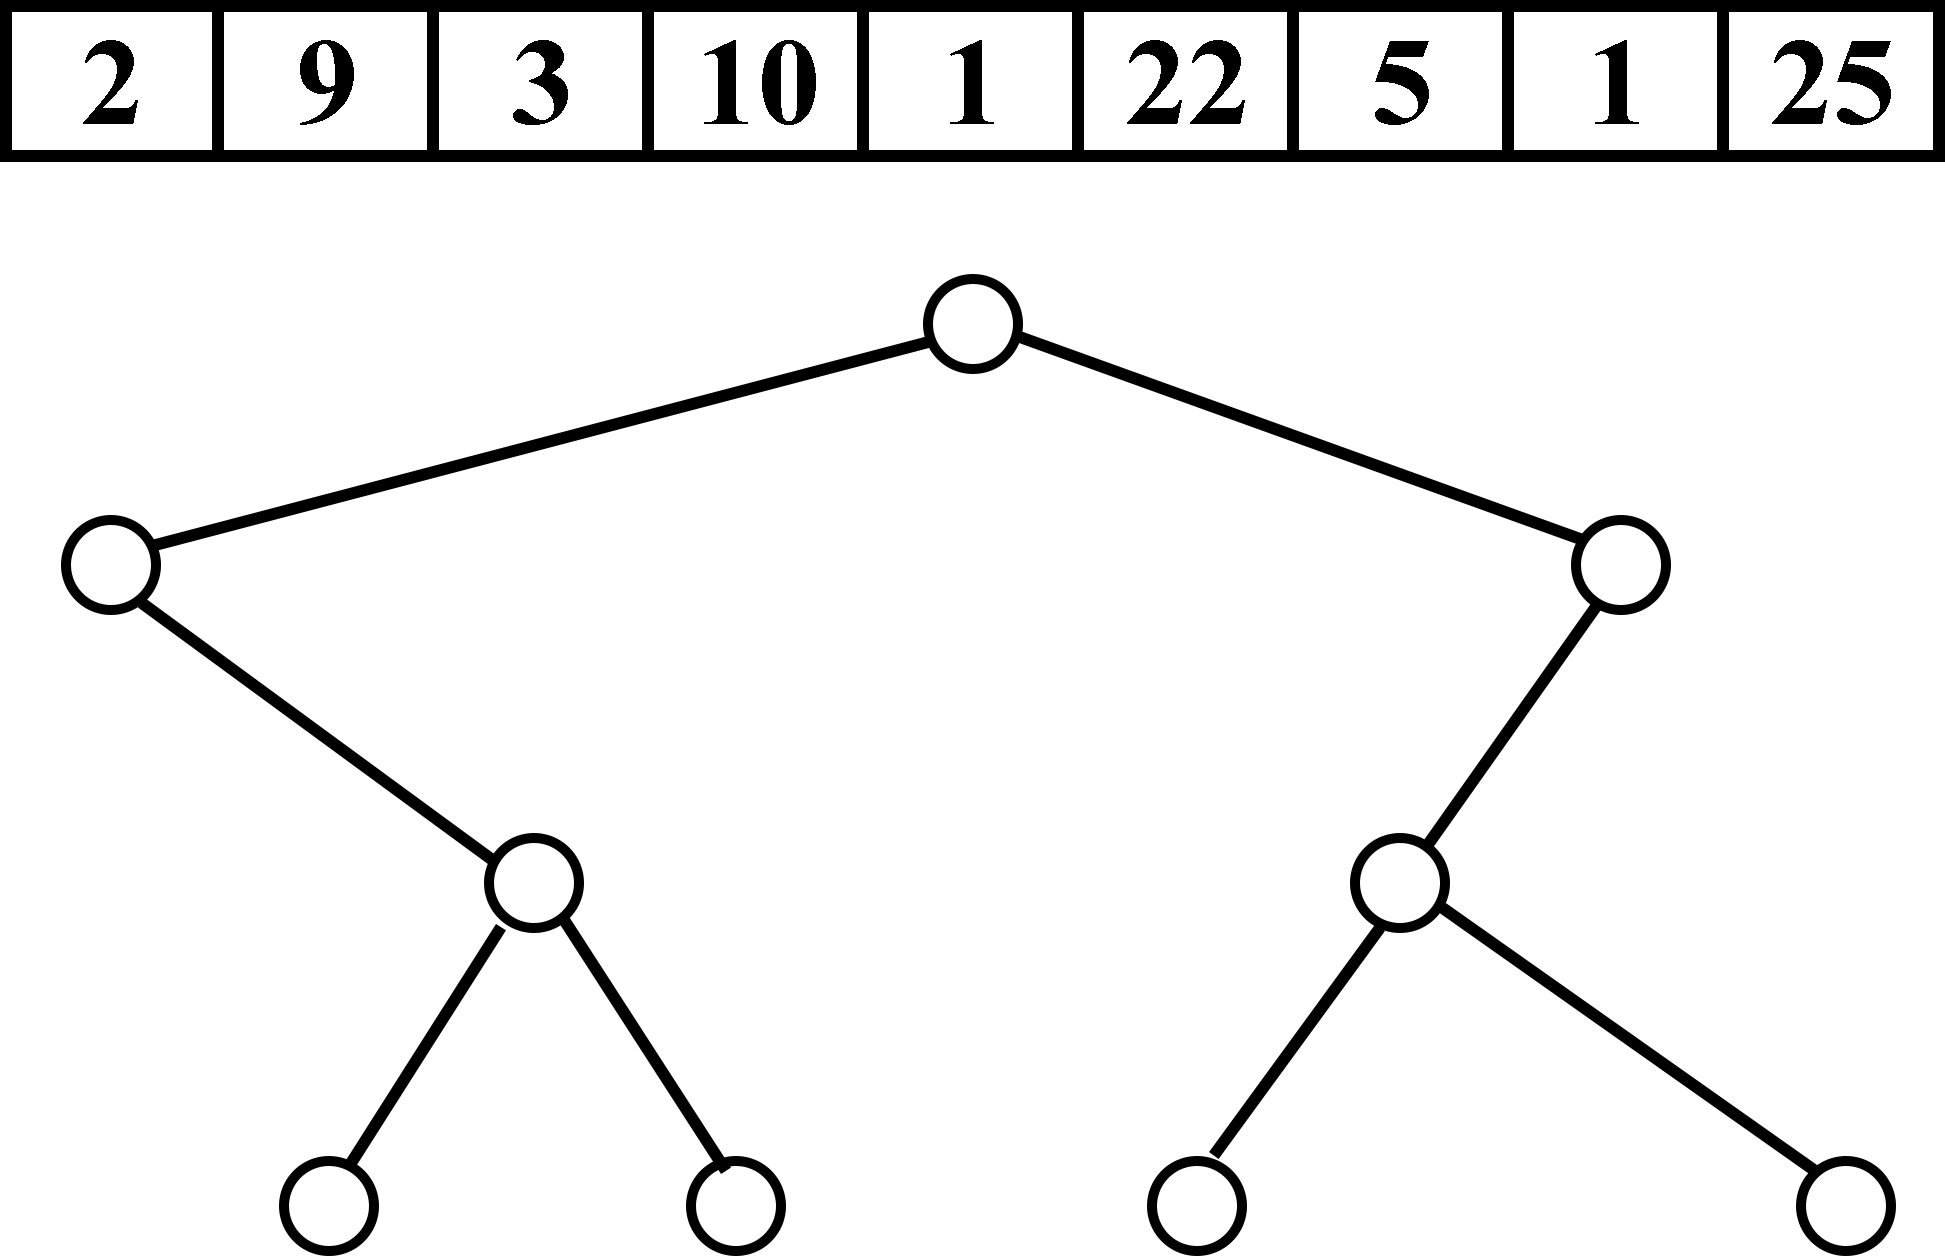
\includegraphics[width=0.6\textwidth]{pic/cartesian-tree-idea.png}
\caption{Пример декартова дерева}\label{fig:cartesian-idea}
\end{figure}

Декартово дерево выполняет базовые операции, такие как вставка, удаление, поиск элемента, 
разрезание и склеивание, в среднем за $O(\log n)$~\cite{cartesian-tree}. Декартовые деревья, построенные 
из последовательности различных чисел обладают следующими свойствами: узлы в декартовом дереве 
соответствуют элементам в исходной последовательности, то есть каждый элемент в последовательности 
соответствует единственному узлу в дереве, каждый узел в дереве также соответствует единственному 
элементу в последовательности. Используя упорядоченный обход, можно вывести исходную 
последовательность чисел: любой нижний индекс элемента из последовательности, 
представленной в левом поддереве дерева узла меньше, чем нижний индекс элемента из последовательности, 
представленной узлом, любой нижний индекс элемента из последовательности, представленной в правом 
поддереве дерева узла больше, чем нижний индекс элемента из последовательности, представленной 
узлом.

\subsection{Параллельный алгоритм вычисления префиксных сумм}

Параллельный алгоритм вычисления префиксных сумм является одним из наиболее важных 
<<кирпичиков>> для параллельной работы с данными~\cite{sengupta06}.
Оно было введено в~\cite{hillis86}.
Данный алгоритм вычисляет все префиксные суммы по данному массиву чисел.
Идея алгоритма приведена на листинге~\ref{listing-prefix-sums}.

\begin{algorithm}[h!]
	\caption{Алгоритм параллельного вычисления префиксных сумм}\label{listing-prefix-sums}
	\begin{algorithmic}[1]
		\For {($j$:=1 to $\log n$ do)}
			\For {(all $k$ in parallel do)}
				\If {$k \ge 2^j$}
   					\State{x[$k$] := x[$k - 2^(j-1)$] + x[$k$]}
  				\EndIf
			\EndFor
		\EndFor
	\end{algorithmic}
\end{algorithm}

Асимтотическая сложность данного алгоритма при использовании $O(N)$ процессоров при работе с 
массивом размера $N$ составляет $O(\log n)$. На рисунке~\ref{fig:prefix-sum} показан пример работы
параллельного алгоритма вычисления префиксных сумм.

\begin{figure}[!ht]
\centering
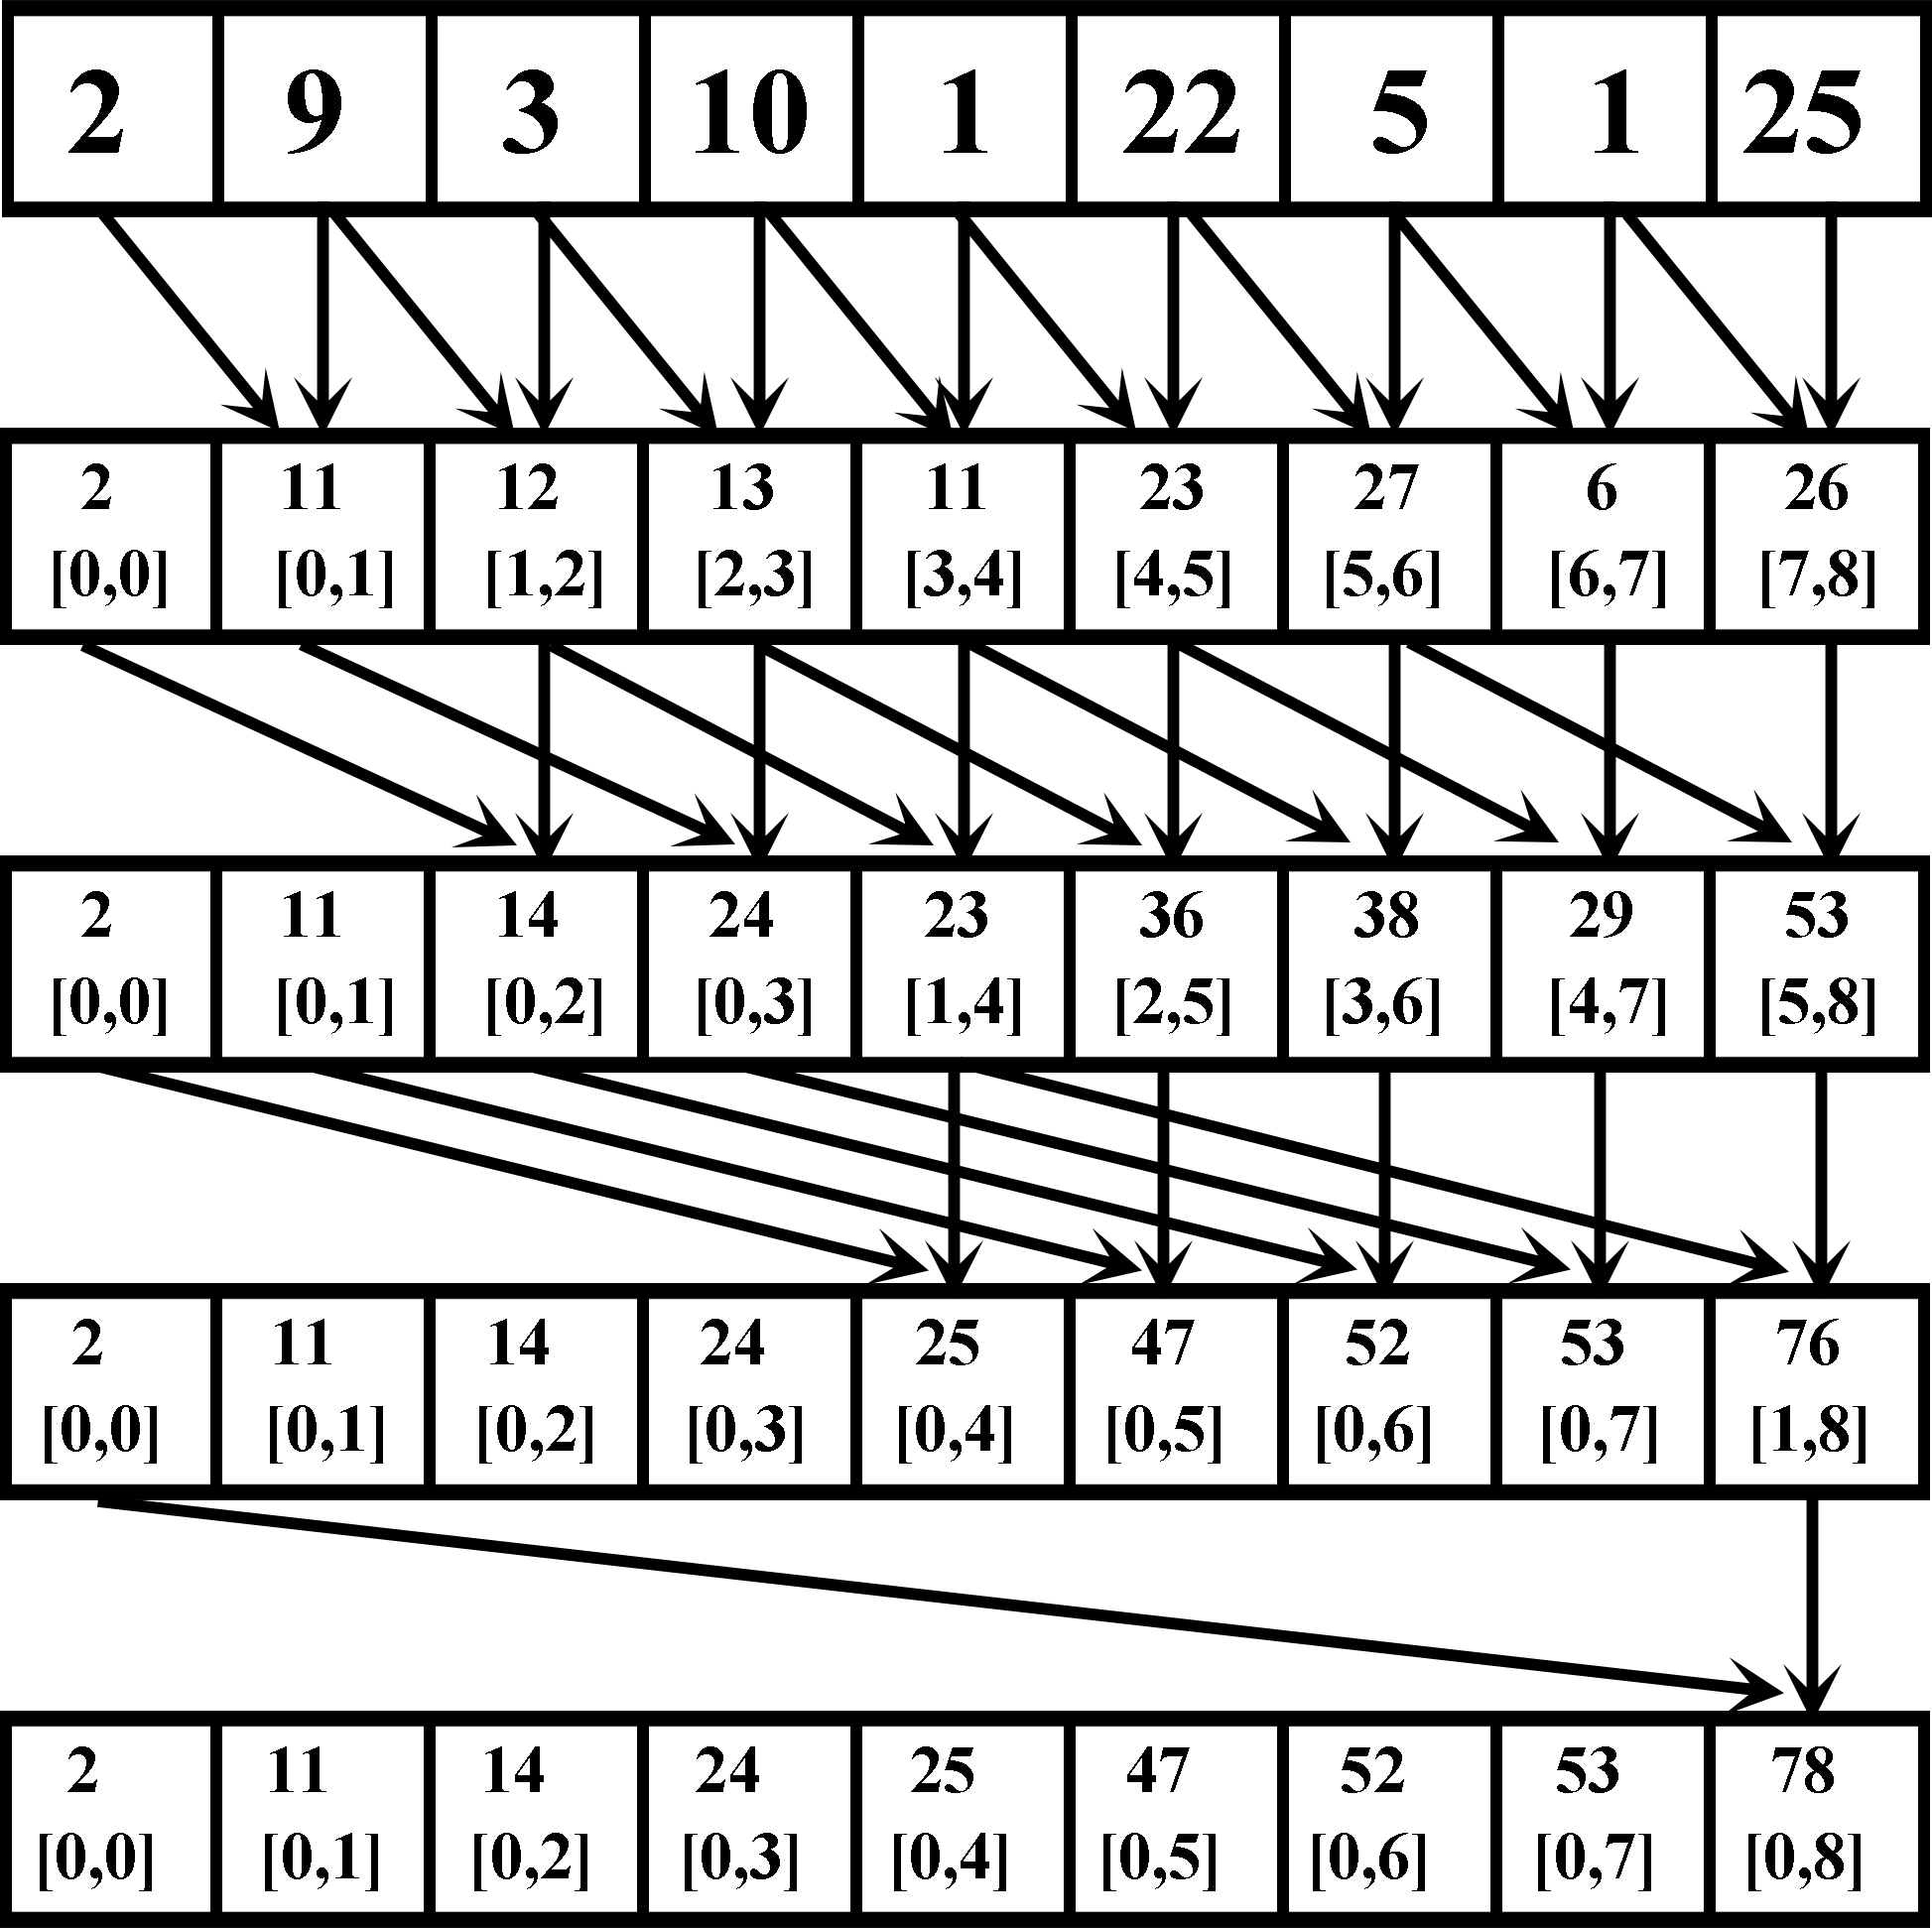
\includegraphics[width=0.7\textwidth]{pic/parallel-prefix-sum.png}
\caption{Иллюстрация идеи параллельного алгоритма вычисления префиксных сумм}\label{fig:prefix-sum}
\end{figure}

\chapterconclusion

В главе приведен обзор методов решения задач поддержания динамических деревьев, алгоритмов параллельного сжатия деревьев, а также некоторых вспомогательных алгоритмов и структур данных. 
В частности, подробно рассмотрены RC-Trees и показана необходимость разработки динамического алгоритма их перестроения. Описаны принципы построения декартова дерева, а также параллельный алгоритм вычисления префиксных сумм, что необходимо для разработки требуемого алгоритма. 

\chapter{Постановка задачи}

Проблемы исследования заключаются в том, что структура данных может быть использована для достижения поставленных целей и то, какие ограничения существуют и каков алгоритм, основанный на структуре данных решающих задачи динамического дерева. В результате обзора литературы, структуры данных сжатия параллельного дерева не достаточно для решения исследовательской задачи, потому что необходима эффективная структура 
динамического дерева данных. Для того, чтобы ответить на динамические запросы и продлить параллельную обработку, должна быть разработана эффективная динамическая структура дерева данных. Сравнивая динамические структуры дерева данных, RC-Trees имеют особенности, которые имеют так же ST-Trees, Topology Tree и Top Tree. RC-Trees улучшенные по Acar U. et al.(2003) использующие распространение изменения могут поддержать изменения в обновлении. В результате, структура данных RC-Trees подходит как базовая структура данных, используемая для покрытия дополнительных изменений в параллельной 
обработке.

Особенность RC-Trees сама по себе требует дополнительного осуществления RC-Trees, таким образом, первое улучшение должно завершить реализацию RC-Trees. Во-вторых, структура данных RC-Trees нуждается в более 
технически продвинутой реализации, чтобы сделать код пригодным для использования в современных приложениях. В-третьих, RC-Trees в параллельном процессе недостаточно эффективны, реализация должна сделать параллельный процесс в каждом Rake и Compress. Другими словами, в каждом вычислительном раунде каждая операция Rake должна выполняться 
параллельно, так же как и операция Compress. Тогда Rake и Compress должны выполняться параллельно.

Кроме того, в настоящее время в теории RC-Trees и структура не поддерживают данные некоммутативного типа, например, матрицы. Таким образом, в реализации и улучшении эта функция должна быть добавлена, и лучше поддержать направленные и ненаправленные данные тоже. Структура данных должна работать эффективно и с простыми данными и с данными больших объемов.


\section{Требования к реализации структуры данных}


Задачи исследования заключаются в необходимости решить то, как структура данных может быть использована для достижения поставленных целей и какие ограничения существуют и каков алгоритм, основанный на структуре данных 
решения задач динамических деревьев. В частности, выбранная структура данных должна поддерживать динамические запросы с постепенными изменениями. По причине того, что текущая работа состоит в том, чтобы структура данных работала в параллельной обработке, следует ответить какие данные параллельных вычислений идут на поддержку структуры. Тогда следующая проблема, если структура данных уже выбрана, заключается в том, что алгоритм должен быть выбран так, чтобы заставить структуру данных работать. 

По сравнению с перечисленными структурами данных, RC-Tree cтруктура данных пригодна. Она поддерживает динамическое дерево и сжатие 
параллельного дерева. Она вцелом способна решить задачи, и RC-Tree cтруктура данных представленая  Acar.U. поддерживает изменения в процессе обновления. RC-Trees реализуют алгоритм сжатия параллельного дерева, включая Rake и Compress. Распространение изменения делает возможным поддержку дополнительных изменений.

Хотя первоначальная структура данных RC-Tree в основном отвечает требованиям для решения исследовательской задачи, но она не поддерживает коммутативные и некоммутативные данные. Кроме того, направленные ребра с 
информацией может оказаться сложными для вычислений. Сложность структуры данных ограничивает расширение для переключения на параллельные вычисления. Ограниченная степень RC-Tree поддерживает не все виды деревьев в лесу.

В результате, RC-Trees не удовлетворяют поставленной задаче, и новая структура данных должна быть разработана на основе RC-Trees и должна поддерживать коммутативные и некоммутативные данных. Для того, чтобы избежать 
ограничения для ограниченной степени, вспомогательная структура может быть использована для изменения исходного дерева в используемое и хранимое дерево. В следующих разделах будет описана разработка новой структуры данных.


\section{Интерфейс для запросов и модификаций}


Новая структура данных, разрабатываемая в данной работе должны поддерживать динамические деревья, так что операции выполняются в лесу. В пользовательском слое  должен быть создан корневой лес, потому что все запросы основаны на этом лесу. В корневом лесу, есть корневые деревья, такие что каждая вершина в лесу имеет корень. В общем, вершина, которая не имеет родителя является корнем. Как правило, в динамическом 
дереве, алгоритм в основном поддерживает запросы на получение номера вершин, ребер и корней в лесу. Кроме того, алгоритм поддерживает запросы к вершине на число её детей, возвращает его родителя, проверяя, если он является корнем, получает информацию, которую она несет, или несут её ребра. 
Вершина несет информацию о самой себе, которая в этой диссертации называется информацией вершины, а 
также информацию о её реберах, которые соединяют её с родителем или детьми, которая называется информация ребра. Информация о вершине поддерживает коммутативную информацию и отвечает на запросы о 
поддереве. Информация о ребре имеет две части, вверхнюю информацию, которая направлена к родителю, и низнюю информацию, которая исходит от детей. Ребра могут нести гораздо больше информации, чем 
вершины, при этом ребра предназначены для поддержки как коммутативный и некоммутативную информации.



В реализации алгоритма, существуют три основных интерфейса поддерживающие ответы на запросы о динамическом дереве: получить корень, получить путь и получить поддерево. Интерфейс для получения корня ищет родителя вершины, от которой был сделан запрос. В случае, если родитель вершины не является корнем, рекурсивно запрашивается родитель родителя вершины и таким образом в конечном счете находится корневая вершина дерева. Данная операция занимает O (1) времени. Интерфейс, отвечающий на запрос пути, возвращает сводную информацию о ребрах на пути между двумя вершинами запроса. Очевидно, что только если две вершины расположены в одном и том же дереве, путь между ними может быть найден. Для того, чтобы получить путь, если две вершины находятся в одном и том же маленьком поддереве, то просто нужно сделать несколько шагов навстречу друг другу, вверх и вниз соответственно, пока 
они не встретятся; если две вершины не в одном и том же маленьком поддереве, они должны дойти до самого нижнего по уровню общего предка. Чтобы получить поддерево вершины нужно добавить информацию о его 
поддереве и нем самом. Ясно, что в RC-Tree только вершина, которая не является корнем, и которая должна быть сжата имеет поддерево, информация о поддереве является объединением информации ее ребенке 
и поддереве этого ребенка.



Чтобы отвечать на динамические запросы более эффективно, был добавлен механизм расписаний, который обновляет дерево в расписании. Каждый раз, когда некоторые изменения сделаны в лесу, он будет проверять, если изменения могут быть сделаны. Каждое изменение может быть записано, но, покуда изменения не внесены в расписание, изменения не будут внесены в лес. 
Операции, производиные пользователями, будут вызывать функцию расписания. Так же они могут вносить сведения о параметрах вершины или ребра. Так же ребра между двумя вершинами могут быть подключены или удалены. Изменения, сделанные 
в дереве могут быть отменены или применены, функция отмены обновляет дерево, как и другие операции, применение функции выполняет все изменения, сделанные на дереве и, наконец, изменяет дерево. Функция расписаний делает последующую параллельную работу более интуитивной и удобной. 
Для ускорения вычислений при использовании функции расписаний, параллельные операции выполняются в функции, когда 
применяемая функция вызывает их.

\chapterconclusion

В главе приводится постановка задачи разработки эффективной структуры данных, поддерживающей инкрементальные изменения. 
Сформулированы требования к реализации структуры данных, описан интерфейс для запросов и модификаций. 

\chapter{Разработка структуры данных}

\section{Снятие ограничения на степень вершины}

В этой диссертации предполагается, что каждая вершина в лесу имеет не более трех детей. Установка ограничения на степень используется для более простого 
вычисления. В бинарном дереве каждая вершина имеет не более двух детей, третий ребенок используется для внутренней структуры данных, используемой для 
выполнения вычислений.

Пользователи могут создавать любые деревья, динамическое дерево не обязано быть бинарным. В этой диссертации, внутреннее дерево --- декартово дерево, 
используется для того чтобы хранить фактические данные. Когда выполняется операция присоединения, она обращается к декартову дереву, чтобы соединить две 
вершины. В декартовом дереве, индекс вершины не совпадает с индексом вершины в представленном дереве, а информация о ребре будет храниться в ребенке в типе 
данных вершины. Например, вершина v, в декартовом дереве имеет индекс 2v. Вершина в декартовом дереве не влияет на вершину в представленном дереве, но 
содержит информацию о ней. Дочерняя вершина в представленном дереве будет располагаться в поддереве его родителя в декартовом дереве. Каждое изменение в 
представленном дереве, такие как вложение, отсоединение и добавление информации о вершине будет вызывать изменение декартового дерева, необходимое для 
обновления фактического сохраненного дерева.

Основной проблемой имеющихся реализаций является константное ограничение на максимальную степень вершины~\cite{acar04}. В настоящей работе его предлагается преодолевать
с помощью следующего приема. Каждая вершина оригинального дерева разбивается на две вершины~--- \emph{вершину данных} (или <<нижнюю>> вершину) и \emph{вершину связей} (или <<верхнюю>> вершину).
Вершина данных всегда имеет родителем соответствующую вершину связей. При этом все дети той или иной вершины организуются в двоичное дерево поиска, корнем которого служит вершина данных родителя, а
остальными вершинами~--- вершины связей детей. В качестве двоичного дерева поиска использовалось декартово дерево~\cite{cartesian-tree}. При таком подходе степень каждой вершины не превосходит трех, что
позволяет использовать алгоритмы для вершин с константной степенью. На рисунке~\ref{fig:represented} приведено оригинальное дерево и дерево, получающееся путем удвоения вершин и организации детей каждой
вершины в виде дерева.

Каждая вершина оригинального дерева снабжена меткой, тип которой является коммутативным моноидом, при этом структура данных поддерживает операцию <<вычислить моноидную сумму меток всех вершин в поддереве
данной вершины>>. Аналогично, каждое ребро оригинального дерева снабжено двумя метками (метка, соответствующая направлению от ребенка к родителю, или <<вверх>>, и аналогичная метка <<вниз>>),
тип которых совпадает и является моноидом (возможно, некоммутативным), при этом структура данных поддерживает операцию <<вычислить моноидную сумма меток всех ребер на пути от вершины $A$
к вершине $B$ для данных вершин $A$ и $B$>>. При удвоении вершин, метки вершин и ребер, выходящих вверх из вершин оригинального дерева, переходят в соответствующие метки соответствущих вершин данных,
в то время как метки вершин и выходящих вверх ребер у вершин связей равны нейтральным элементам соответствующих моноидов. Таким способом достигается корректность выполнения запросов независимо от
структуры деревьев, организующих детей вершин.

\begin{figure}[!ht]
\centering
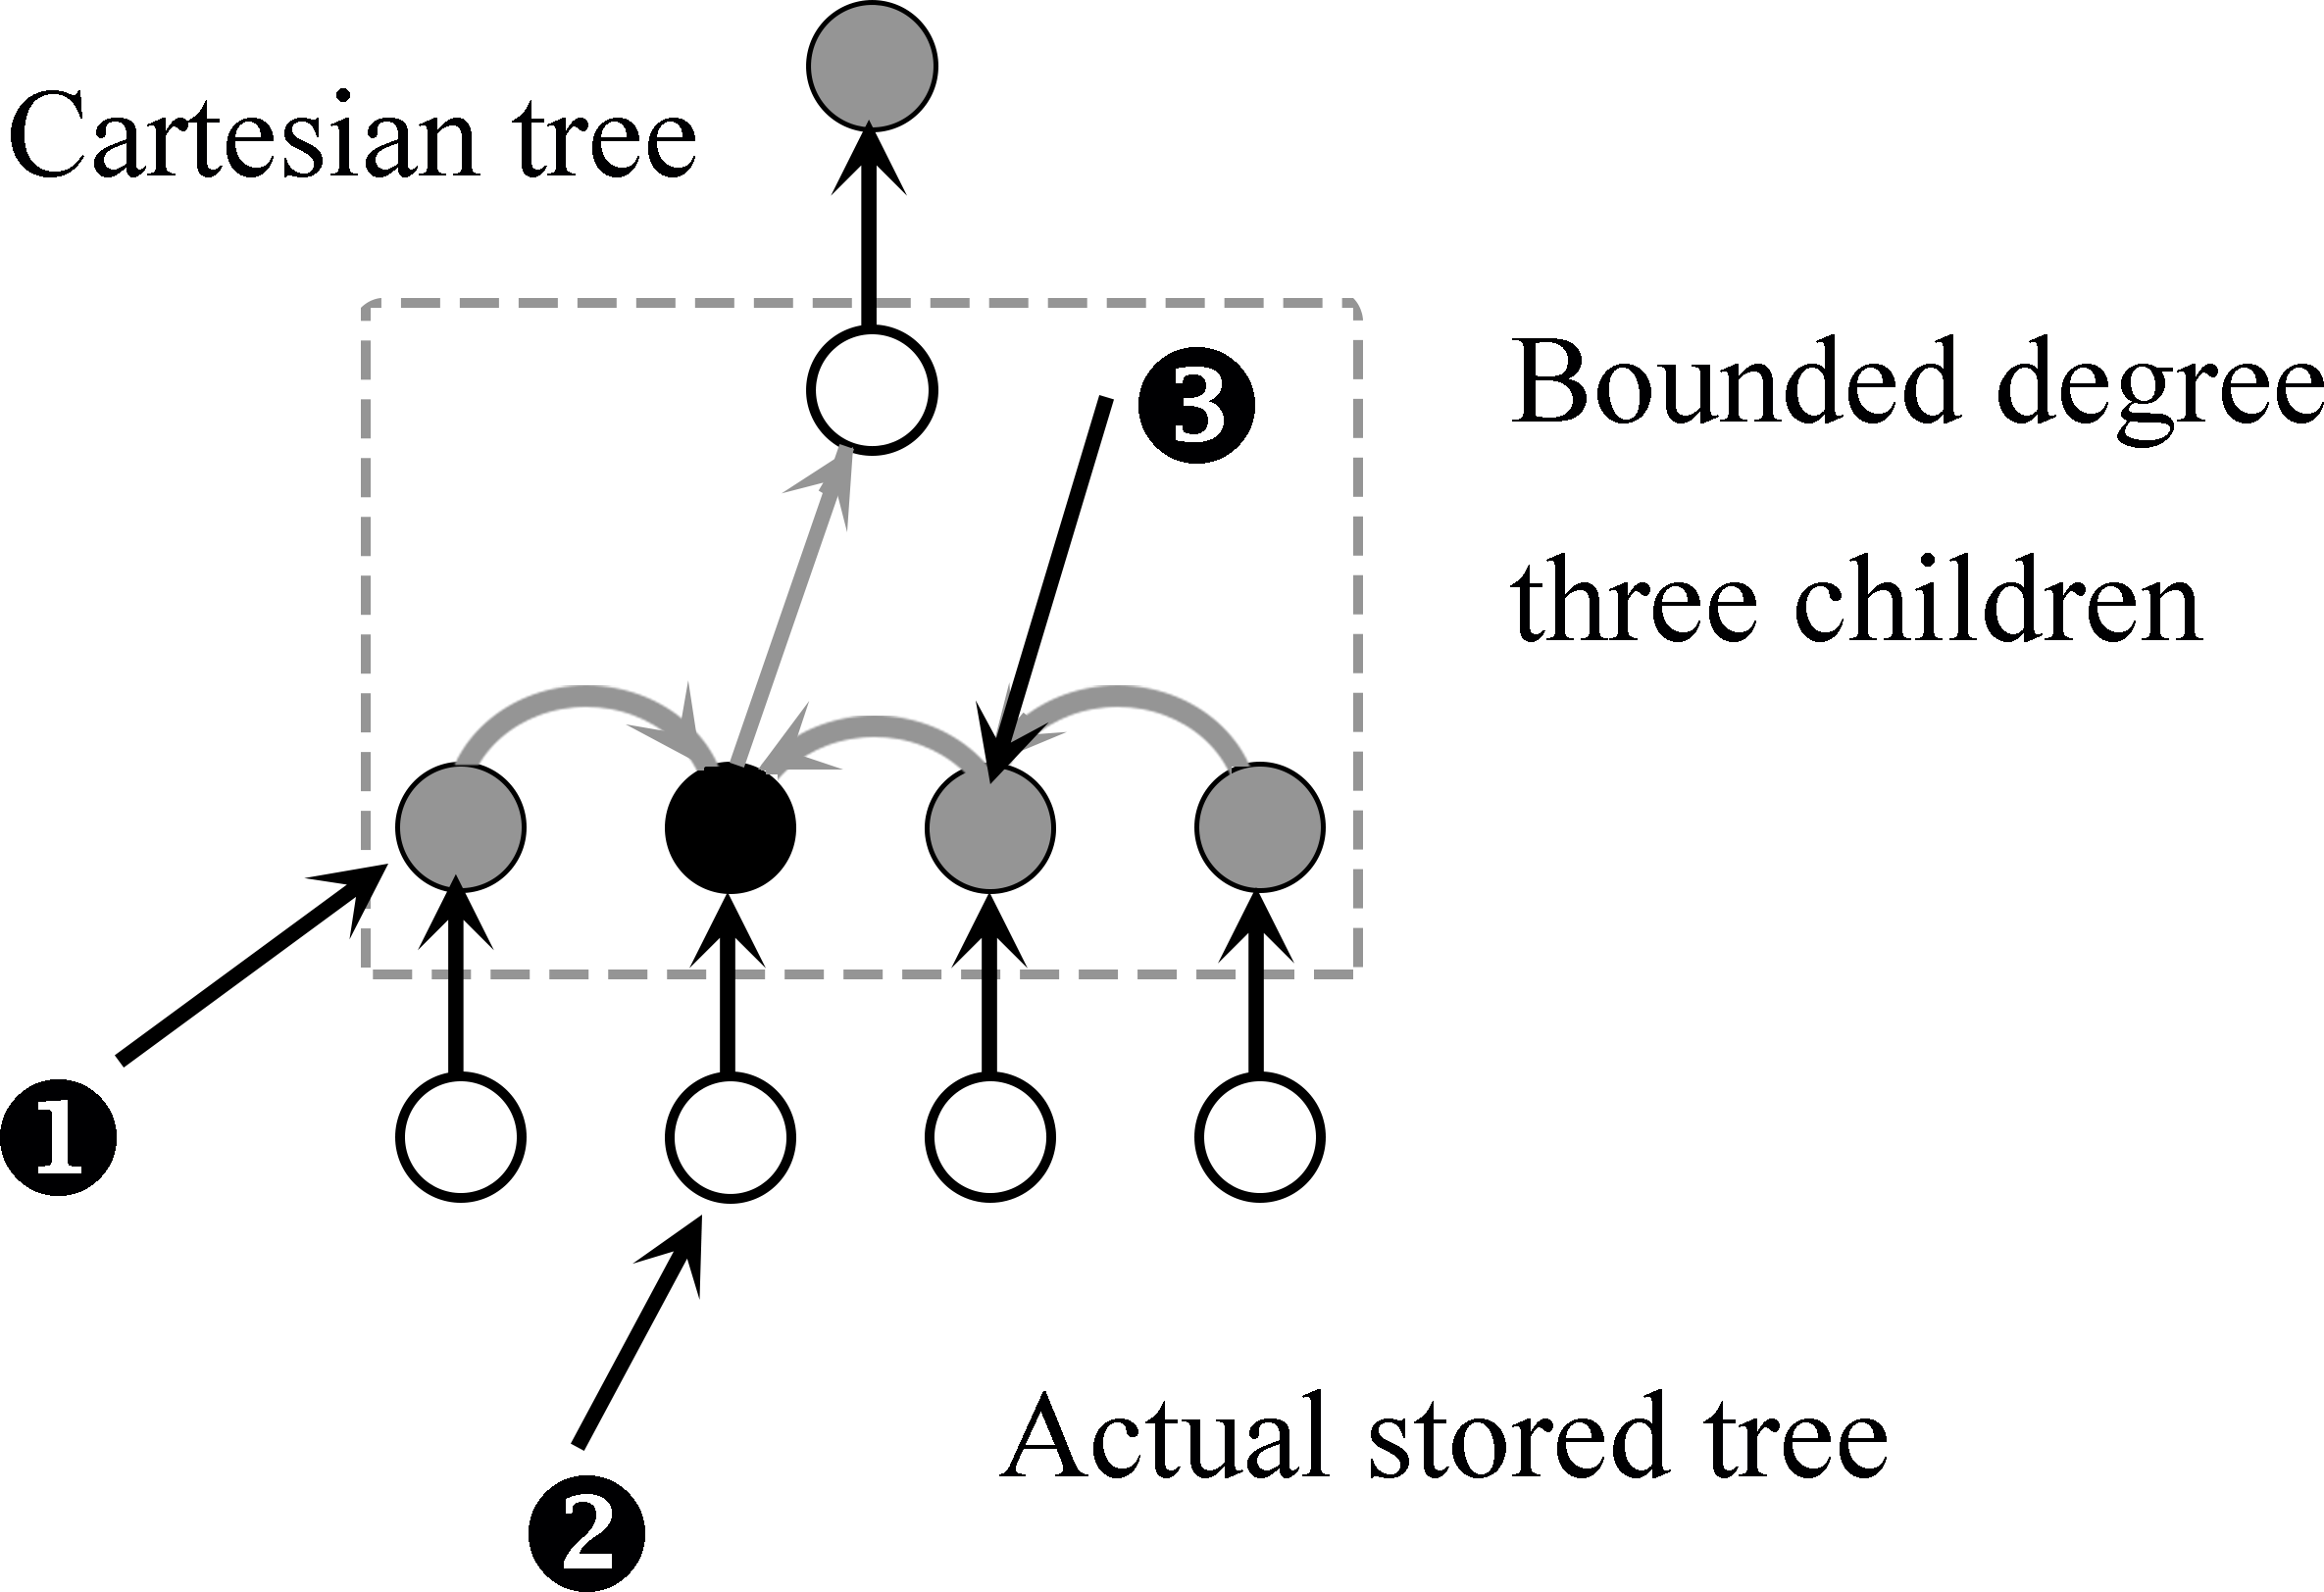
\includegraphics[width=0.55\textwidth]{pic/Cartesian_tree.png}
\caption{Представление вершины и ее детей с помощью декартова дерева}\label{fig:cartesian-children}
\end{figure}

\begin{figure}[!ht]
\centering
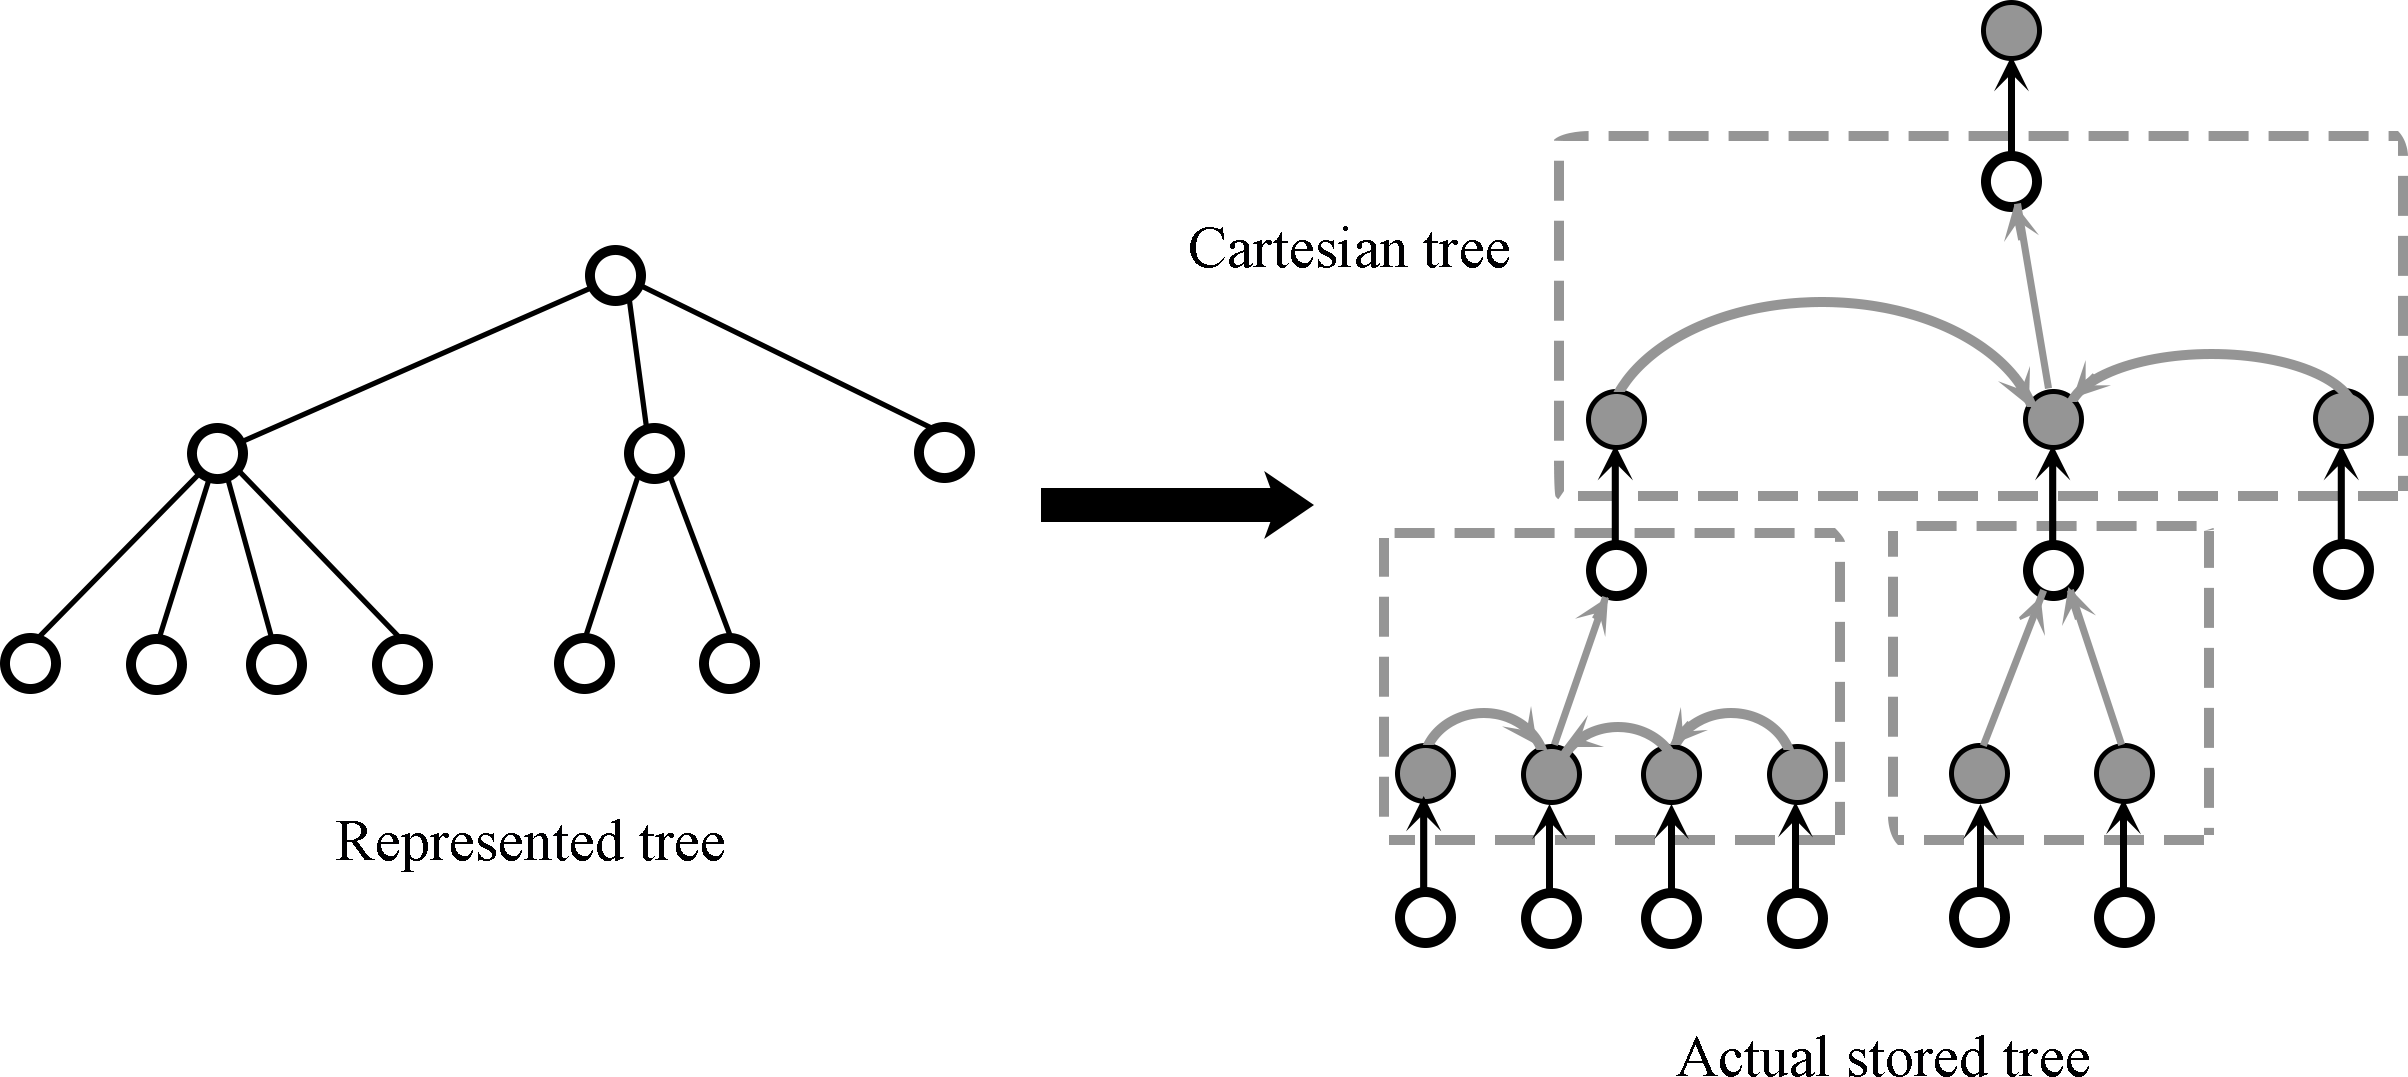
\includegraphics[width=1.0\textwidth]{pic/represented_tree_and_actual_stored_tree.png}
\caption{Исходное RC-дерево и дерево, которое хранится в памяти}\label{fig:represented}
\end{figure}

%Исходный код реализации дерева, а также нижеследующих экспериментов, располагается в репозитории GitHub по адресу
%\url{https://github.com/feng7/pasl/tree/pdt/example/rc-tree}.

\section{Хранение данных с использованием $O(N)$ оперативной памяти}


Структура данных, разработанная в диссертации, поддерживает операции динамических изменений. Рассмотрим механизм использования структуры данных расписания. Уровни используются для разъяснения операций. 
В каждой вершине хранится структура данных типа <<столбец>>, в которой записывается каждое изменение вершины, как показано на рисунке. Все новые созданные вершины на первом уровне структуры, как только 
они меняются, выталкиваются на следующий уровень, это выглядит как во второй матрице. Вершины типа столбца имеют свою информацию об уровне. В результате упрощается проверка последнего активного
уровня, в котором вершина может корректно выполнять операции.


\begin{figure}[!ht]
\centering
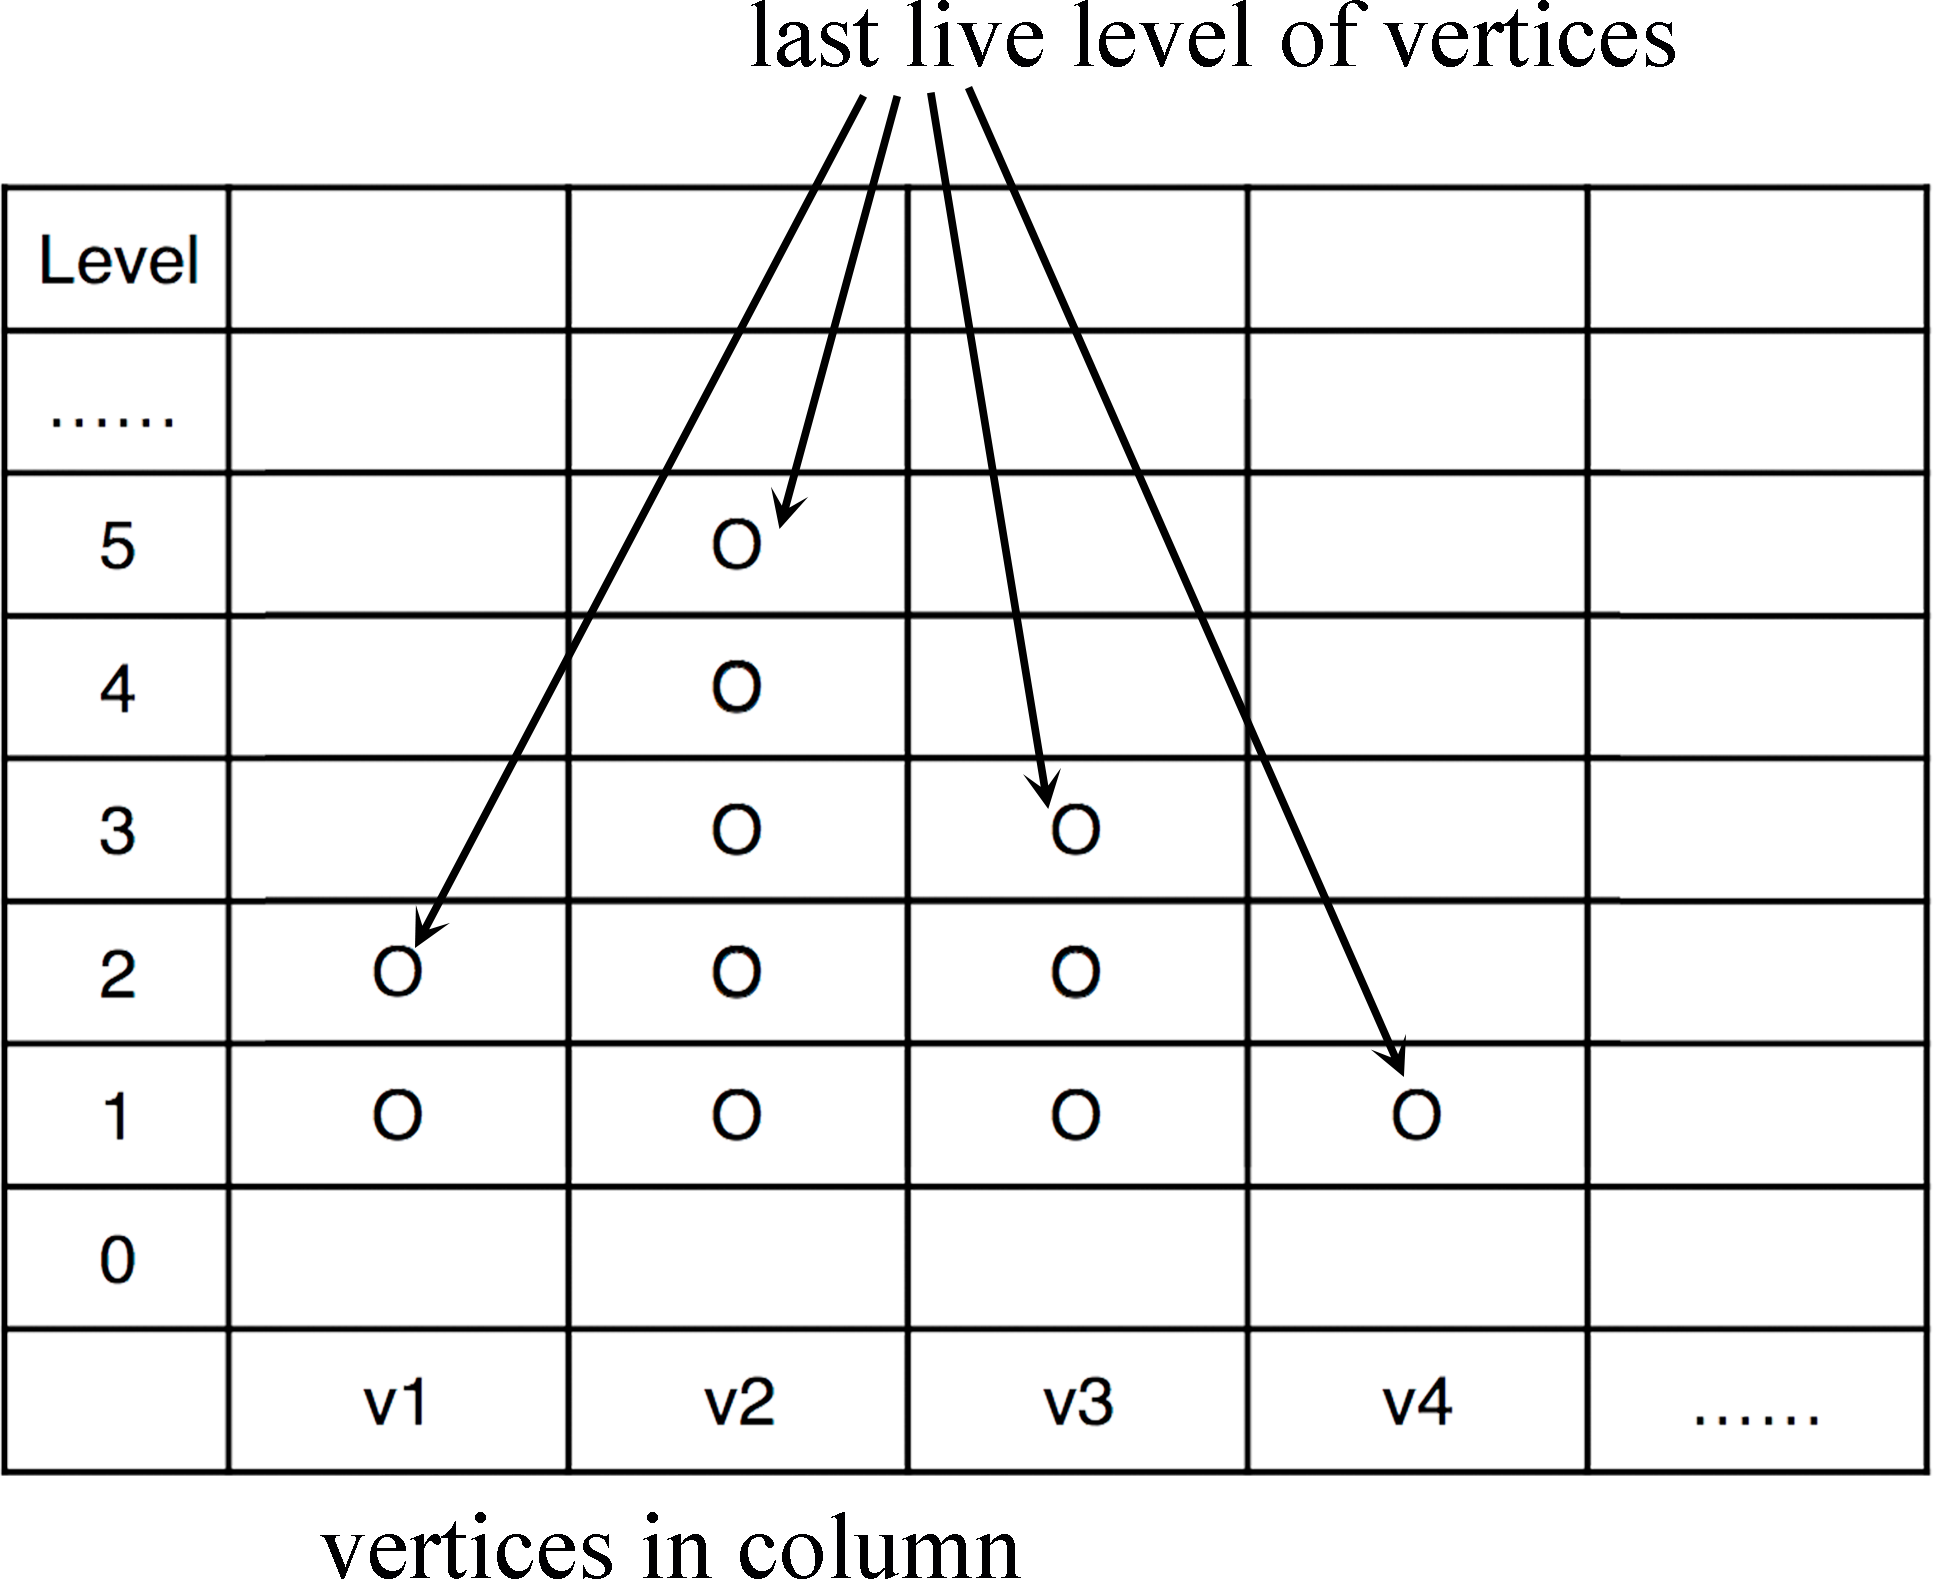
\includegraphics[width=0.7\textwidth]{pic/vertices_in_column.png}
\caption{Хранение данных c использованием $O(N)$ оперативной памяти}\label{fig:memory}
\end{figure}

\section{Проверка применимости модификаций}

Для того, чтобы избежать ошибочных операций, сделанных на дереве, предлагается интерфейс для проверки ошибок динамической связи. Как правило, операции, 
выполняемые на динамическом дереве с двумя вершинами, требуют проверки их отношений. Операция проверки связи и проверки соединения между двумя вершинами проверяют, связаны ли вершины между собой или не связаны, 
но находятся в одном дереве. Проверка занимает $O (\log n)$ времени каждый раз, когда вызывается операция обновления, однако она не всегда необходима. 
Например, при операции отсоединения достаточно проверить только, является ли родительская вершина корнем. В операции разрезания необходимо проверить степень первой вершины, так как операция может быть выполнена только если вторая вершина является ее ребенком. Таким образом, проверка ошибок во время операции отсоединения занимает от $O (\log n)$ до $O (\log d)$, где $d$ является степенью родителя.

\section{Применение обновлений}

Как уже упоминалось выше, уровни используются для обозначения модифицированных вершин на каждом раунде операций. Когда вызывается операция, последние использованные вершины вершины размещаются на
нулевом и первом уровнях. Затем выполняется цикл, чтобы применить операции на каждом уровне. В соответствии с числом модифицированных вершин, вызывается функция обработки вершины. Функция проверяет 
состояние вершины, если текущая вершина является последней активной вершиной в его колонке, то 
функция будет выполнять операции Rake, Compress или другие изменения непосредственно. Eсли текущая вершина не 
активна, происходит рекурсивный вызов функции и текущая вершина перемещается на следующий уровень. Иными словами, функция фактически обновляет динамическое дерево. После обработки вершин одного уровня, необходимо проверить число следующих затрагиваемых вершин, чтобы обновить числа следующих затрагиваемых вершин текущей вершины на следующем уровне.

Перед тем, как внести изменения, необходимо проверить, применима ли операция к вершине. Функция \texttt{will{\textunderscore}*} проверяет, станет ли вершина корнем, или к ней будут применены операции Rake или compress, или вершина будет изменена, но может участвовать в Rake или Compress на следующем уровне. Если результат проверки положительный, то функция \texttt{do{\textunderscore}*} выполняет необходимые операции. Если 
вершина подвергается операции Rake, 
это влияет на ее родителей, и число ее следующих затрагиваемых вершин должно быть увеличено на единицу. Если к вершине применяется операция compress, эта операция влияет как на ее родителей, так и на детей. Однако поскольку фактически используется декартово дерево, будет затронут только первый ребенок. В остальных случаях вызывается обработка вершин на следующем уровне.

\section{Реализация параллельных вычислений}

Как уже упоминалось выше, параллельное вычисление сделано в цикле с помощью вызова функции обработки вершины из расписания. Функция обработки обходит уровни для проверки всех измененных или посещенных вершин. 
Параллельные вычисления будут работать на каждом уровне для каждой вершины. В 
результате в новом алгоритме, разработанном в данной работе, на каждом уровне операции Rake, 
compress, turn to root, а также другие необходимые операции, выполняются параллельно, 
когда они находятся на том же уровне. Каждое изменение на определенном уровне будет влиять на следующий уровень, поэтому лучше не выполнять операции на разных уровнях параллельно.

%!!!!!!   Непереводимая игра слов
%Looping drivers are used in the data structure, it makes easier to switch parallel methods. In the apply function, change the loop function to driver function, and the compute prefix sum function as well. For comparison, the looping driver performs in sequential uses the common loop function.
%В структуре данных используются специальные функции, облегчающие переключение параллельных методов. При применении операции, измените зацикливающую функцию  для функции водителя, а функция Compute prefix 
%sum, а также. Для сравнения, зацикливание драйвер выполняет в последовательном использует функцию общего цикла.

\chapterconclusion

В главе описана разработанная структура данных. Представлен механизм снятия ограничения на степень вершины, описаны принципы хранения данных с использованием $O(n)$ оперативной памяти. 
Разработана процедура проверки применимости модификаций. Описано, как происходит применение обновлений. Приводится описание реализации параллельных вычислений. 

\chapter{Экспериментальное исследование}

Ранее была описана разработка алгоритма, в этом разделе рассматриваются эксперименты для оценки его эффективности. Время работы последовательной реализации оценивается как базовая величина для сравнения со временем работы параллельной реализации. Для параллельной обработки данных используются две библиотеки, PASL и OpenMP. Они также сравниваются друг с другом. Эксперименты запускаются на компьютере с 4 ядрами процессора и 4 Гб памяти.

\section{Тестовые сценарии}

Эксперименты по измерению времени построения разработанной реализации и выполнения ею запросов производятся на следующих тестах:
\begin{enumerate}
    \item дерево-<<палка>>: $n$ вершин, при этом $i$-тая вершина является ребенком $(i-1)$-ой вершины при $i > 0$.
    \item дерево-<<пучок>>: $n$ вершин, при этом $i$-тая вершина является ребенком вершины 0 при $i > 0$.
    \item дерево-<<два пучка>>: $n$ вершин при $n = 2m$, $m$ целое, при этом вершина 0 является родителем вершин с 1 по $(m-1)$,
          вершина $m$ является родителем вершин с $(m+1)$ по $(n-1)$, а вершины 0 и $m$ дополнительно соединены.
    \item построение дерева-<<палки>> в десять этапов, каждый из которых состоит в присоединении $n / 10$ вершин.
\end{enumerate}

\section{Экспериментальное исследование последовательной реализации}

Выполнено четыре теста: 
\begin{itemize}
\item построение $n$ вершин линейного дерева --- тест 1 <<длинная цепь>>; 
\item построение $n$ вершин дерева-<<пучка>> --- тест 2 <<большая степень>>; 
\item построение двух деревьев-<<пучков>> с $n$ вершинами --- тест 3  <<две большие степени>>; 
\item построение дерева-<<палки>> с десятью уровнями, в каждом из которых соединены $n/10$ вершин --- тест 4 <<инкрементальная длинная цепь>>.
цепью. 
\end{itemize}
Рассматриваются различные значения числа вершин. Каждый раз после построения дерева из $n$ вершин выполняется $n$ запросов к поддеревьям и $n$ запросов к путям. 
В таблице приведено время работы структуры данных на тестах. Средняя сложность алгоритма составляет $O (\log n)$.

\begin{table}[!ht]
\centering
\begin{tabular}{|l|l|l|l|l|}\hline
 & $n=10000$ & $n=100000$ & $n=1000000$ & $n=3000000$ \\\hline
1 & 0.063533 & 0.936087 & 9.8946 & 31.3906 \\\hline
2 & 0.031963 & 0.473844 & 5.04014 & 16.8301 \\\hline
3 & 0.03333 & 0.495401 & 5.19158 & 16.8656 \\\hline
4 & 0.068615 & 0.840358 & 11.1828 & 36.3289 \\\hline
\end{tabular}
\caption{Результаты экспериментов для последовательной реализации}\label{tbl:results-seq}
\end{table}

\section{Экспериментальное исследование реализации с использованием OpenMP}

Оценим время работы параллельной реализации с применением OpenMP. Используются те же тесты, что и для последовательной реализации.
Тем не менее, OpenMP может использовать процессоры с различным числом ядер. Проводятся тесты, 
проверяющие эффективность OpenMP на числе процессоров 1, 2, 4 и 8.

Параллельный метод с использованием OpenMP применяется в зацикливающей функции. Перед циклом добавляется строка 
\texttt{\#pragma omp parallel for schedule (guided, 100)}. 
Для функции compute prefix sum сначала параллельно вычисляются предварительные значения; затем 
производится проверка, достигнут ли конец цикла и начинается ли последовательно следующий цикл, 
чтобы убедиться, что можно использовать предварительно посчитанные значения. Проверка выполняется 
в одном потоке. В таблицах~\ref{tbl:results-openmp-1}--\ref{tbl:results-openmp-8} показано время 
работы, полученное с использованием OpenMP.

\begin{table}[!ht]
\centering
\begin{tabular}{|l|l|l|l|l|}\hline
 & $n=10000$ & $n=100000$ & $n=1000000$ & $n=3000000$ \\\hline
1 & 0.07072 & 1.01285 & 11.4329 & 35.1043 \\\hline
2 & 0.033578 & 0.48801 & 5.46487 & 17.5146 \\\hline
3 & 0.035731 & 0.515872 & 5.68942 & 18.0354 \\\hline
4 & 0.075208 & 0.891592 & 12.389 & 40.6775 \\\hline
\end{tabular}
\caption{Результаты экспериментов для OpenMP, один процессор}\label{tbl:results-openmp-1}
\end{table}

\begin{table}[!ht]
\centering
\begin{tabular}{|l|l|l|l|l|}\hline
 & $n=10000$ & $n=100000$ & $n=1000000$ & $n=3000000$ \\\hline
1 & 0.081845 & 1.10473 & 11.6696 & 35.7506 \\\hline
2 & 0.04275 & 0.510112 & 5.47687 & 18.0637 \\\hline
3 & 0.044991 & 0.529194 & 5.59677 & 17.8966 \\\hline
4 & 0.11298 & 1.00143 & 12.9886 & 41.9446 \\\hline
\end{tabular}
\caption{Результаты экспериментов для OpenMP, два процессора}\label{tbl:results-openmp-2}
\end{table}

\begin{table}[!ht]
\centering
\begin{tabular}{|l|l|l|l|l|}\hline
 & $n=10000$ & $n=100000$ & $n=1000000$ & $n=3000000$ \\\hline
1 & 0.089218 & 1.22818 & 13.169 & 40.9343 \\\hline
2 & 0.07859 & 0.553611 & 5.78005 & 18.871 \\\hline
3 & 0.047683 & 0.583647 & 5.94402 & 18.8319 \\\hline
4 & 0.159757 & 1.12068 & 14.4973 & 47.2622 \\\hline
\end{tabular}
\caption{Результаты экспериментов для OpenMP, четыре процессора}\label{tbl:results-openmp-4}
\end{table}

\begin{table}[!ht]
\centering
\begin{tabular}{|l|l|l|l|l|}\hline
 & $n=10000$ & $n=100000$ & $n=1000000$ & $n=3000000$ \\\hline
1 & 0.103436 & 1.61389 & 17.3962 & 54.0412 \\\hline
2 & 0.067749 & 0.638183 & 6.74281 & 21.2547 \\\hline
3 & 0.072668 & 0.638638 & 7.00279 & 21.7108 \\\hline
4 & 0.340943 & 1.39135 & 17.9712 & 58.4357 \\\hline
\end{tabular}
\caption{Результаты экспериментов для OpenMP, восемь процессоров}\label{tbl:results-openmp-8}
\end{table}

\section{Экспериментальное исследование реализации с использованием PASL}

Эксперименты проводятся аналогично экспериментам для OpenMP, однако в случае PASL тестируется также возможность использования процессоров с различным числом ядер. 
Параллельный метод с использованием PASL применяется в цикле. Используется инструкция 
\texttt{pasl::sched::native::parallel{\textunderscore}for}. Для функции compute prefix sum сначала 
параллельно вычисляются предварительные значения; затем производится проверка, достигнут ли конец 
цикла и начинается ли последовательно следующий цикл, чтобы убедиться, что можно использовать 
предварительно посчитанные значения. В таблицах~\ref{tbl:results-pasl-1}--\ref{tbl:results-pasl-8} 
показано время работы, полученное с использованием PASL с различным числом процессоров.

\begin{table}[!ht]
\centering
\begin{tabular}{|l|l|l|l|l|}\hline
 & $n=10000$ & $n=100000$ & $n=1000000$ & $n=3000000$ \\\hline
1 & 0.073684 & 1.09323 & 12.3956 & 38.1296 \\\hline
2 & 0.036832 & 0.522955 & 5.75152 & 18.5603 \\\hline
3 & 0.038104 & 0.548474 & 6.03994 & 19.1851 \\\hline
4 & 0.078299 & 0.953348 & 13.0366 & 42.883 \\\hline
\end{tabular}
\caption{Результаты экспериментов для PASL, один процессор}\label{tbl:results-pasl-1}
\end{table}

\begin{table}[!ht]
\centering
\begin{tabular}{|l|l|l|l|l|}\hline
 & $n=10000$ & $n=100000$ & $n=1000000$ & $n=3000000$ \\\hline
1 & 0.141362 & 1.61106 & 15.5824 & 47.6541 \\\hline
2 & 0.077958 & 0.859135 & 8.91695 & 28.6172 \\\hline
3 & 0.078529 & 0.88774 & 8.77827 & 29.134 \\\hline
4 & 0.155524 & 1.90973 & 18.7348 & 58.2101 \\\hline
\end{tabular}
\caption{Результаты экспериментов для PASL, два процессора}\label{tbl:results-pasl-2}
\end{table}

\begin{table}[!ht]
\centering
\begin{tabular}{|l|l|l|l|l|}\hline
 & $n=10000$ & $n=100000$ & $n=1000000$ & $n=3000000$ \\\hline
1 & 0.28281  & 2.71137 & 22.9835 & 69.6526 \\\hline
2 & 0.149832 & 1.5798 & 14.5509 & 49.3806 \\\hline
3 & 0.162006 & 1.61922 & 14.9153 & 48.653 \\\hline
4 & 0.313789 & 3.73799 & 31.7739 & 93.2229 \\\hline
\end{tabular}
\caption{Результаты экспериментов для PASL, четыре процессора}\label{tbl:results-pasl-4}
\end{table}

\begin{table}[!ht]
\centering
\begin{tabular}{|l|l|l|l|l|}\hline
 & $n=10000$ & $n=100000$ & $n=1000000$ & $n=3000000$ \\\hline
1 & 0.563715 & 5.00583 & 39.7913 & 121.166 \\\hline
2 & 0.306949 & 2.98072 & 27.0531 & 89.4415 \\\hline
3 & 0.322895 & 3.15966 & 28.327 & 87.608 \\\hline
4 & 0.644581 & 7.4977 & 57.6276 & 167.604 \\\hline
\end{tabular}
\caption{Результаты экспериментов для PASL, восемь процессоров}\label{tbl:results-pasl-8}
\end{table}



\section{Сравнение результатов экспериментов}

Эксперимент с последовательной реализацией выполняется в одном потоке. 
На рисунках~\ref{fig:results-comparison-1}--\ref{fig:results-comparison-4} 
показано сравнение времени работы последовательной реализации, OpenMP и PASL. 

\begin{figure}[!ht]
\centering
\begin{subfigure}[b]{0.45\textwidth}
    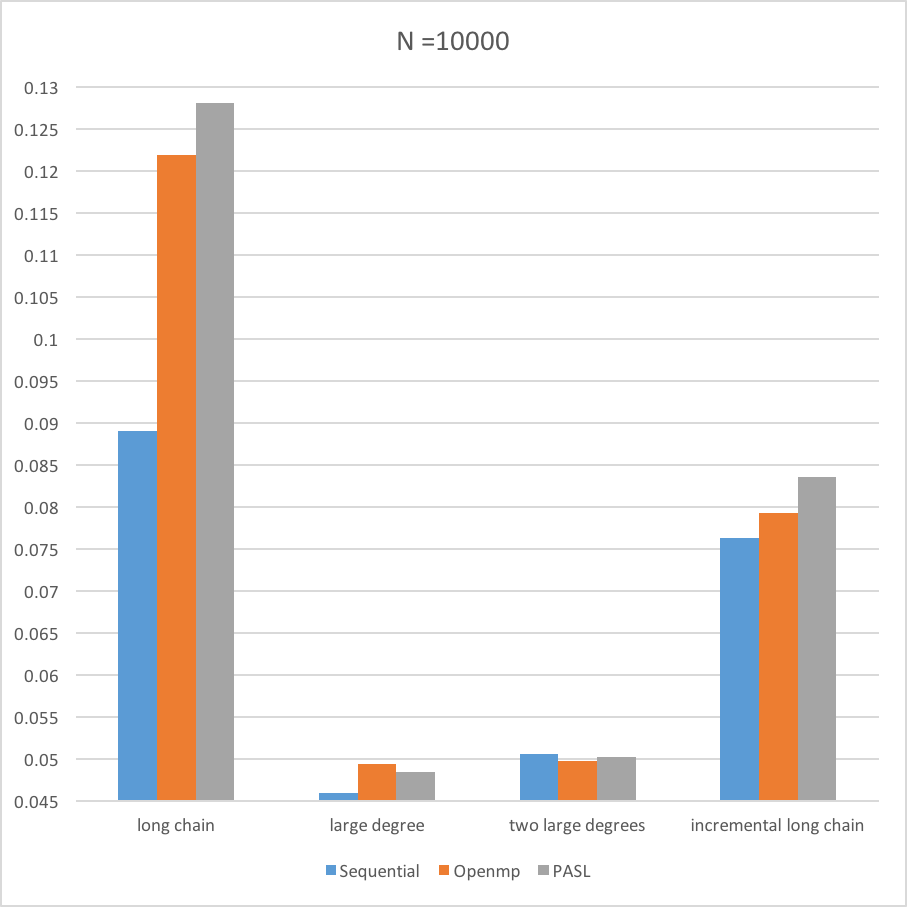
\includegraphics[width=\textwidth]{pic/results-1-a.png}
\end{subfigure}~~\begin{subfigure}[b]{0.45\textwidth}
    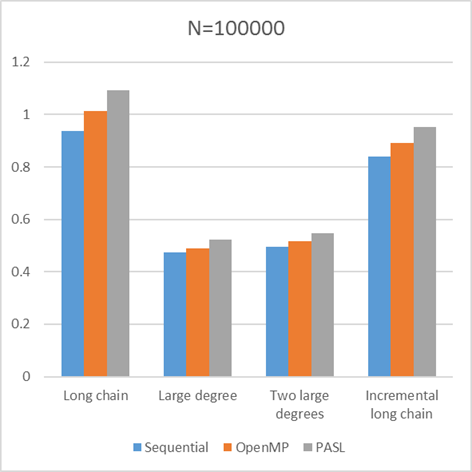
\includegraphics[width=\textwidth]{pic/results-1-b.png}
\end{subfigure}\\
\begin{subfigure}[b]{0.45\textwidth}
    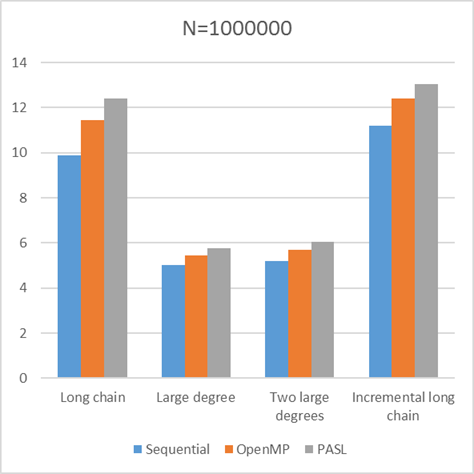
\includegraphics[width=\textwidth]{pic/results-1-c.png}
\end{subfigure}~~\begin{subfigure}[b]{0.45\textwidth}
    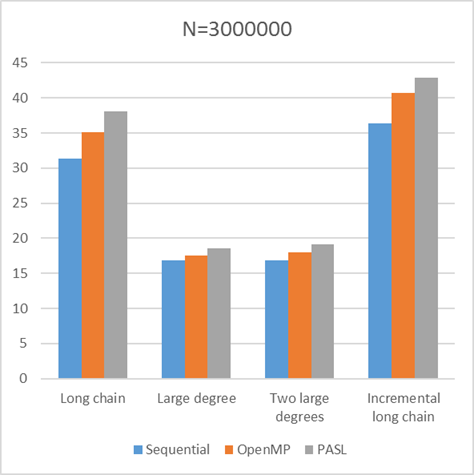
\includegraphics[width=\textwidth]{pic/results-1-d.png}
\end{subfigure}
\caption{Сравнение результатов, один процессор}\label{fig:results-comparison-1}
\end{figure}

На рисунке~\ref{fig:results-comparison-1} высота столбца соответствует времени работы алгоритма. 
Можно видеть, что последовательная реализация в случае использования одного процессора является наилучшей. 
Кроме того, можно видеть, что на тесте <<длинная цепь>> OpenMP занимает меньше времени. В целом, в случае использования одного процессора PASL может занять много времени.

\begin{figure}[!ht]
\centering
\begin{subfigure}[b]{0.45\textwidth}
    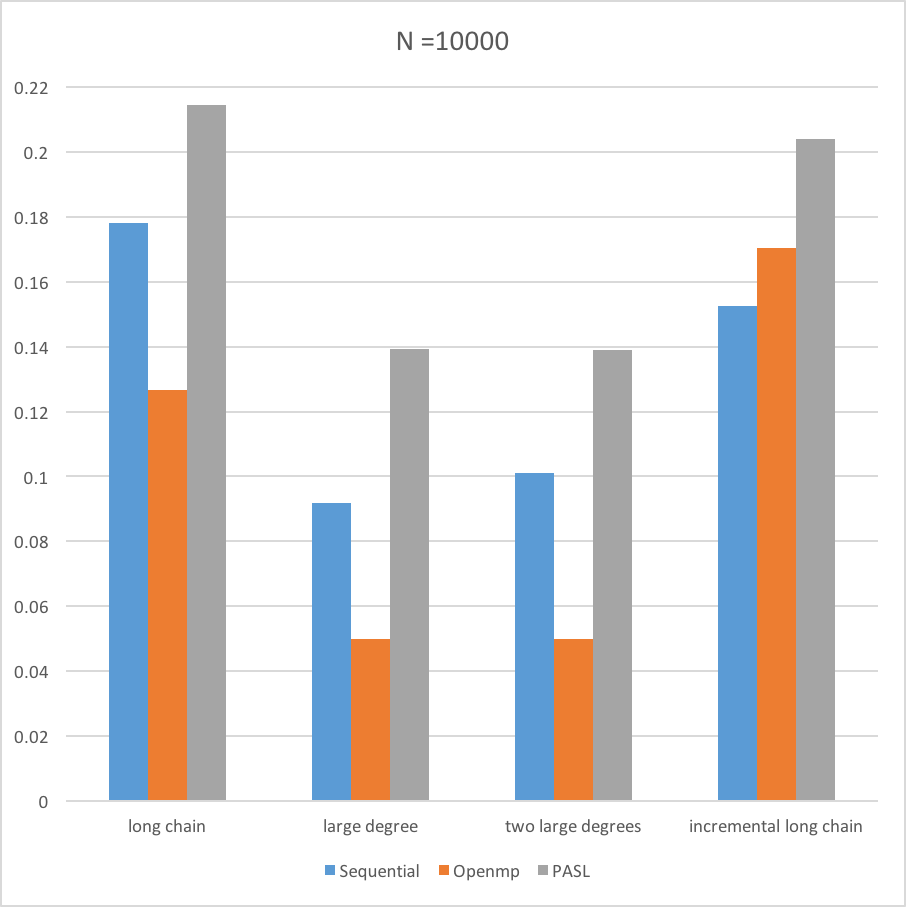
\includegraphics[width=\textwidth]{pic/results-2-a.png}
\end{subfigure}~~\begin{subfigure}[b]{0.45\textwidth}
    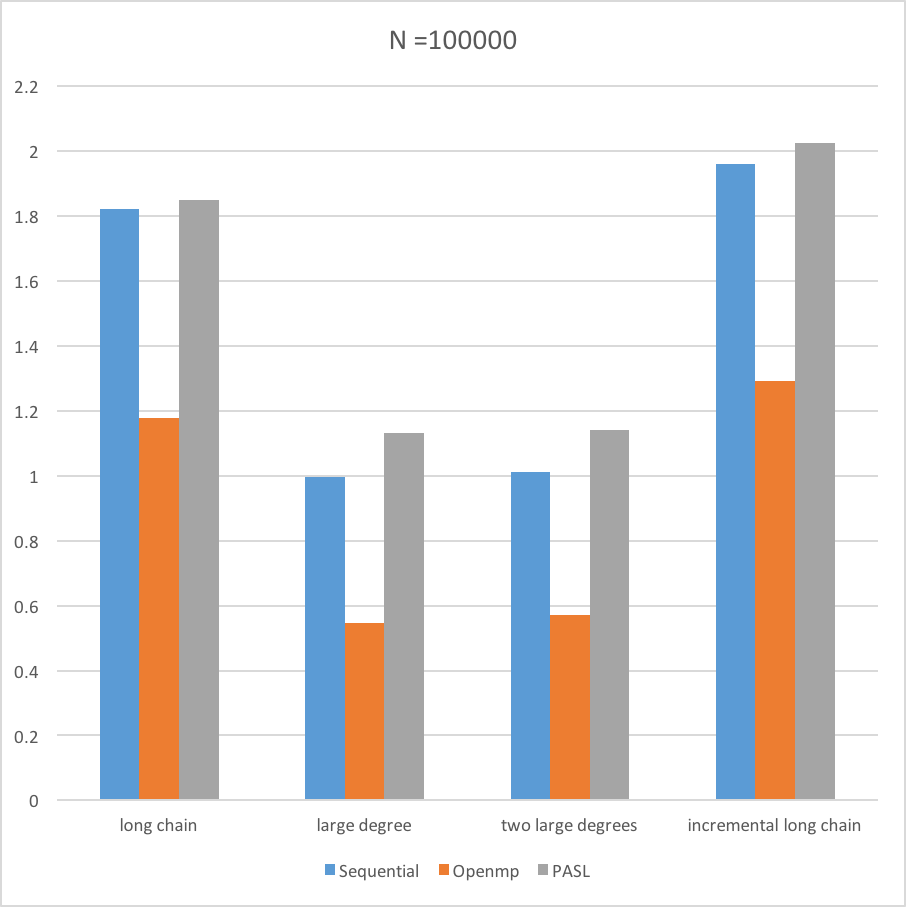
\includegraphics[width=\textwidth]{pic/results-2-b.png}
\end{subfigure}\\
\begin{subfigure}[b]{0.45\textwidth}
    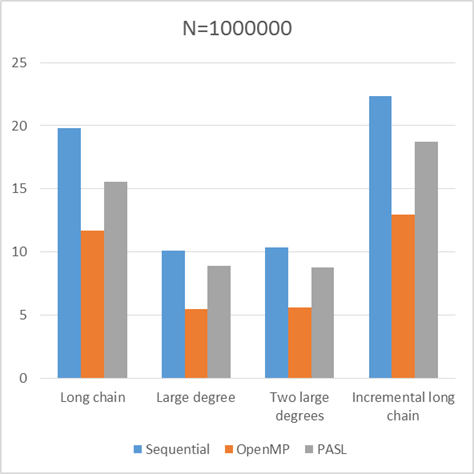
\includegraphics[width=\textwidth]{pic/results-2-c.png}
\end{subfigure}~~\begin{subfigure}[b]{0.45\textwidth}
    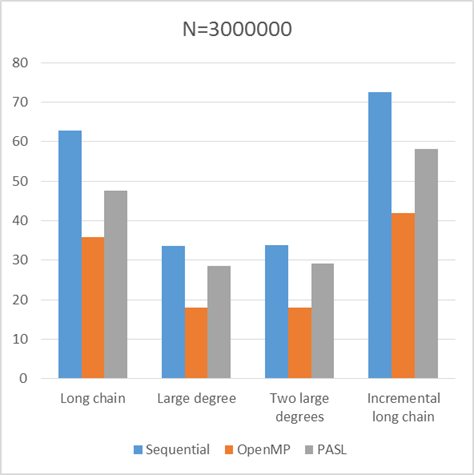
\includegraphics[width=\textwidth]{pic/results-2-d.png}
\end{subfigure}
\caption{Сравнение результатов, два процессора}\label{fig:results-comparison-2}
\end{figure}

\begin{figure}[!ht]
\centering
\begin{subfigure}[b]{0.45\textwidth}
    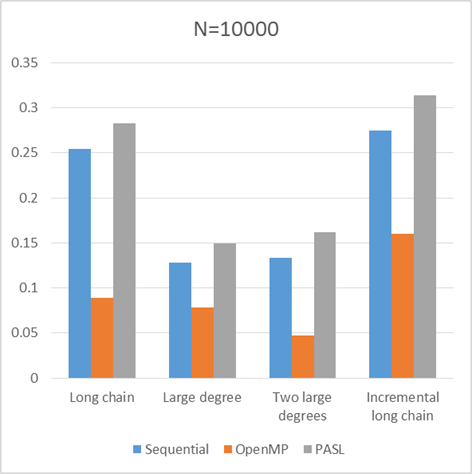
\includegraphics[width=\textwidth]{pic/results-4-a.png}
\end{subfigure}~~\begin{subfigure}[b]{0.45\textwidth}
    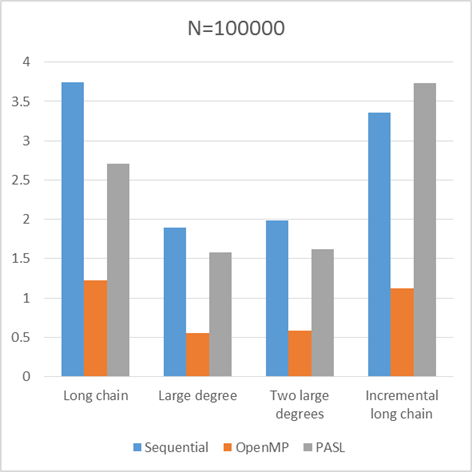
\includegraphics[width=\textwidth]{pic/results-4-b.png}
\end{subfigure}\\
\begin{subfigure}[b]{0.45\textwidth}
    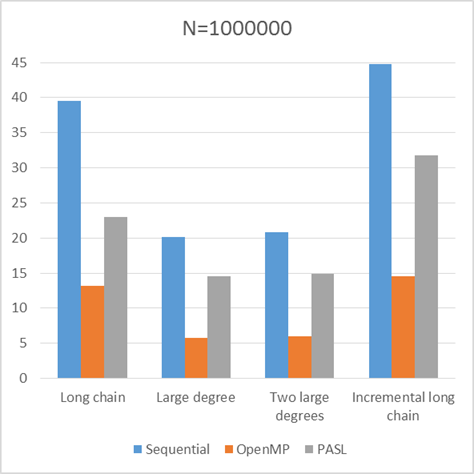
\includegraphics[width=\textwidth]{pic/results-4-c.png}
\end{subfigure}~~\begin{subfigure}[b]{0.45\textwidth}
    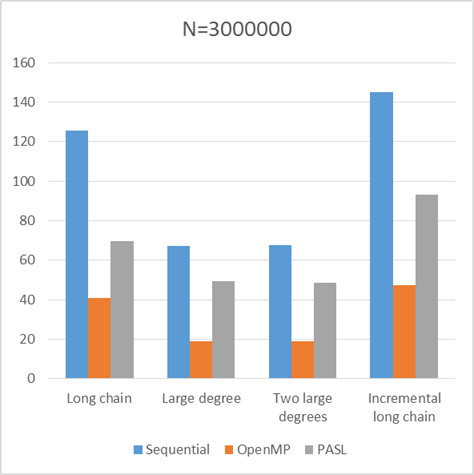
\includegraphics[width=\textwidth]{pic/results-4-d.png}
\end{subfigure}
\caption{Сравнение результатов, четыре процессора}\label{fig:results-comparison-4}
\end{figure}

\begin{figure}[!ht]
\centering
\begin{subfigure}[b]{0.45\textwidth}
    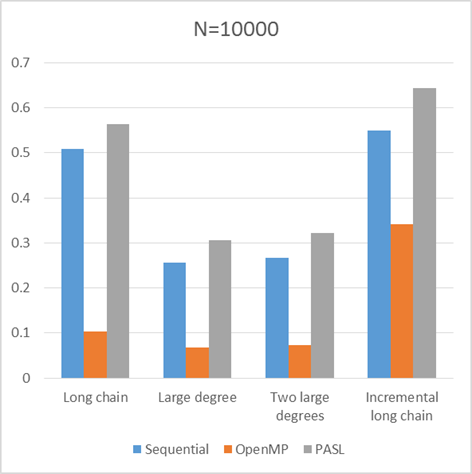
\includegraphics[width=\textwidth]{pic/results-8-a.png}
\end{subfigure}~~\begin{subfigure}[b]{0.45\textwidth}
    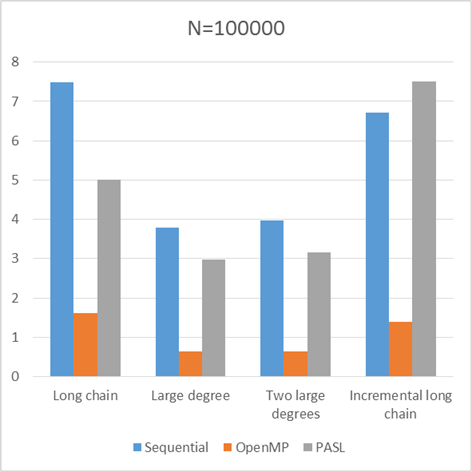
\includegraphics[width=\textwidth]{pic/results-8-b.png}
\end{subfigure}\\
\begin{subfigure}[b]{0.45\textwidth}
    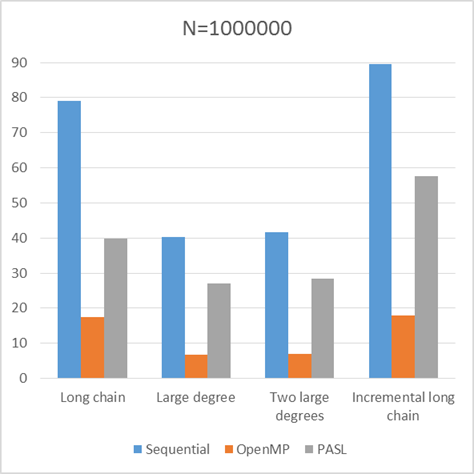
\includegraphics[width=\textwidth]{pic/results-8-c.png}
\end{subfigure}~~\begin{subfigure}[b]{0.45\textwidth}
    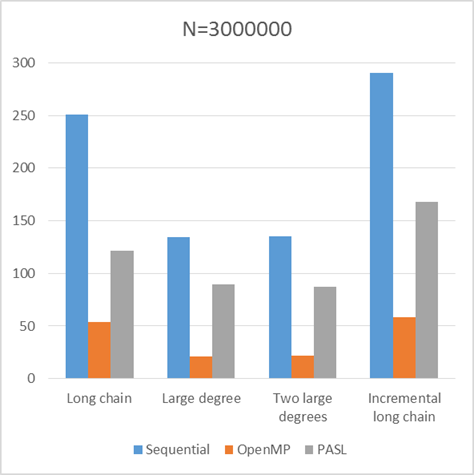
\includegraphics[width=\textwidth]{pic/results-8-d.png}
\end{subfigure}
\caption{Сравнение результатов, восемь процессоров}\label{fig:results-comparison-8}
\end{figure}

На рисунках~\ref{fig:results-comparison-2}--\ref{fig:results-comparison-8} представлены результаты 
в случае использования нескольких процессоров. Можно видеть, что в этом случае OpenMP эффективнее, чем PASL.


\chapterconclusion

В главе описано экспериментальное исследование эффективности предложенной структуры данных, поддерживающей инкрементальные изменения и предназначенной для параллельной обработки деревьев. 
Приводятся использованные тестовые сценарии. Выполняется экспериментальное исследование последовательной реализации, а также параллельных реализаций с использованием OpenMP и PASL. Библиотека PASL позволяет использовать различное число ядер процессора, однако демонстриует низкую производительность в случае использования одного процессора. В большинстве рассмотренных случаев наиболее эффективной является реализация на основе OpenMP. 


%% Макрос для заключения. Совместим со старым стилевиком.
\startconclusionpage

В диссертации предложена структура данных, поддерживающая инкрементальные изменения и предназначенная для параллельной обработки деревьев. Предложенная структура основана на дереве Rake and Compress, а также декартовых деревьях и параллельном алгоритме вычисления префиксных сумм. Реализовано хранение данных с использованием $O(n)$ оперативной памяти, разработана процедура проверки применимости модификаций, поддерживается возможность выполнения параллельных вычислений. 

Эффективность предложенной структуры данных проверяется экспериментально на примере четырех тестовых конфигураций. Производится сравнение с последовательной реализацией, а также исследуется эффективность реализаций на основе PASL и OpenMP. Результаты экспериментов подтверждают эффективность предложенной структуры данных в случае использования OpenMP. 

%% Обратите внимание на heading. Без него тоже работает, но название будет другим.
\printmainbibliography

\end{document}
